%%%%%%%%%%%%%%%%%%%%%%%%%%%
\chapter {Parallel Black Virus Decontamination in Meshes}
\label{DL}
%%%%%%%%%%%%%%%%%%%%%%%%%%%
 
\section{Introduction}
In this chapter, we discuss parallel strategy on BVD problem in grid and tori. In the sequential strategy ({\em BVD-2G}) for 2-dimensional grids which are meshes, an ``explorer agent ''and a ``leader explorer agent'' are sent to explore the graph and locate the BV. They traverse the mesh in a snake-like fashion column by column following the ``casual walk''. In the sequential protocol ({\em BVD-qG}) for q-dimensional grids, the grid is partitioned into $d_1\times\ldots\times d_{q-2}$ 2-dimensional grids of size $d_{q-1}\times d_q$, and each 2-dimensional grid is explored using the shadowed traversal technique as described in the 2-dimensional grids. Similarly, in the protocol ($BVD-qT$) for q-dimensional torus, the torus is partitioned into $d_1\times \ldots \times d_{q-1}$ ring of size $d_q$. The exploration procedure traverses a ring and, when back to the starting point, proceeds to another ring, with a neighbouring starting point. After locating the BV, agents surround the new formed BVs sequentially and eliminate them. These strategies are simple to follow, but at the same time they are not time-efficient. Now we consider that if more than two agents are allowed to participate in the exploring phase and we focus on decreasing the time cost in the exploring phase and the number of casualties, how to design a new strategy so that the we are able to reach the destination with acceptable cost (the increasing number of agents used in the exploring phase).\\
The general idea is simple, we will employ a group of agents and place them in a specific array at the beginning. Informally, in the shadowed exploration of our strategy in 2-dimensional grid({\em PBVD-2G}), q-dimensional grid({\em PBVD-qG})and tori({\em PBVD-qT}), the agents who are employed to explore the graph stay in that array and that ``agent array"  traverse that graph in the shadowed exploration. Note that after the BV is triggered, not all the agents automatically enter the elimination phase but only the agents who know the existence of BV, but in some cases, the number of agents knowing the existence of BV is not enough for surrounding and eliminating the BVs, so in the elimination phase, our strategies employ some agents who receive the clones of the original BV(thus knowing the existence of the BV) to notify some other agents to participate in the elimination phase. 
Also, we compare the number of agents, the time cost, the number of movement and also the casualty between each of our strategy and the sequential strategy.

\section{Parallel BV Decontamination of Grids}
\subsection{Base Case:2-Dimensional Grid}
A 2-dimensional grid (which is a mesh) of size $d_1\times d_2$ has $n=d_1\times d_2(d_1>2,d_2>2)$ nodes. Without loss of generality, let $d_1<d_2$ and let the node of {\em M} be donated by their column and row coordinate ($x_1$,$x_2$), $1\leq x_1 \leq d_1$, $1\leq x_2 \leq d_2$. Observe that in a mesh, we have three types of nodes: \textit{corner} (entities with only two neighbours), \textit{border}(entities with three neighbours), and \textit{interior}(with four neighbours).  Our strategy follows two phases: shadowed exploration and elimination. In the first phase, the network is traversed until the location of the BV is determined. That location is clear after the visit while all of its unprotected neighbours have become BVs. Actually, in $PBVD-2G$, there are only one new formed BV. In the second phase, new formed BV is surrounded and permanently eliminated. Note that when we say the second phase starts, we actually mean that those agents knowing the existence of BV start to surround the BV, or notify some other agents, and then eliminate the BV, but not mean that all the agents enter this phase. There are two significant differences between $PBVD-2G$ and the sequential strategy: the number of agents employed in the exploration phase; the route of agents in the exploration phase. We also give the routes of agents in the elimination phase. 

\noindent{\bf Shadowed Exploration Phase} \\

As we introduce above, we should place the agents in a specific array at the beginning and then let them explore the graph. Now let us consider how to arrange them at the beginning and how to design the routes for them to explore the graph. We prefer to place the agents at the borders (or the corners) of the mesh because in this way we can reduce the casualties. For the same purpose of reducing the casualties, we prefer to arrange all the agents in a array so that when one of the exploring agent trigger the BV, the exploring agents and shadowed agents guide as many neighbours of the BV as possible. In another word, we want all the agent explore the graph in one direction but not from different direction. With these two principles, our strategy in the shadowed exploration is that given specific number of agents, we place them in one border of the mesh and if there are more agents, we place them on the row which is parallel to the border and so on. Then we design routes for them so that at any time they move to one direction to explore the graph. \\
Monotonicity is a principle that we should obey in the whole process, which means one exploring agent should be followed by at least one shadowed agent, so the number of agents in the exploration phase should be at least twice the number of the exploring agents. To guarantee the monotonicity and the two principles, we should employ $2a\,(a\in\mathbb{Z}^*)$ agents in this phase and place $a$ of them in one of the border and the others in the second line paralleling to the border.
Now let's consider the number of agents we should employ.
When $a=1$, the arrangement is actually the sequential case. Since we want to explore the graph parallelly, let's start from the base case when $a=2$. The initial arrangement would be as Fig\ref{fig:twoagent1}:
\begin{figure}[H]
  \centering  
  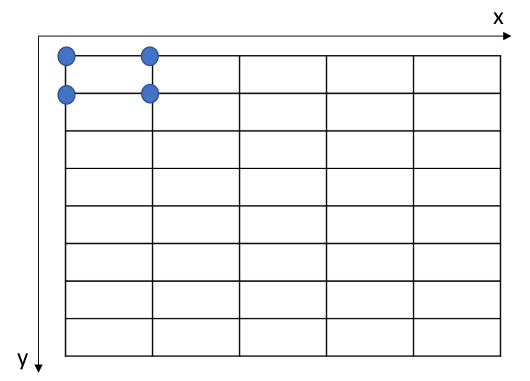
\includegraphics[width=2.5in]{figures/twoagent1.png}
  \caption{Arrangement of agents at the beginning(when $a=2$)}\label{fig:twoagent1}
\end{figure}

Now let's consider the routes for the agents. For convenience, we assume that all the agents move at $T(x)\,(x\in\mathbb{Z}^*)$ because some time should be reserved for the coordination after the BV is triggered. More detail about the moving cycle would be discussed after we decide the number of agents and the routes for them. 
Let $v=(x, y)$ be the node under exploration, with $1\leq x_i \leq d_1$, $1\leq i \leq d_2$. Additionally, we define ``Vertical Moving Mark'' (VMM) for every agent: VMM can only change between $0$ and $1$; every time when the agent moves SOUTH, that value changes. For example, if one agent continues to move SOUTH at $T(x)\,(x\in\mathbb{Z}^*)$ and its $Vertical_D$ is originally $0$, then its $Vertical_D$ changes into $1$ at $T(1)$, $0$ at $T(2)$ and so on.
Every agent hold two VMMs in its memory and let's say $VMM_1$ and $VMM_2$. The original value of $VMM_1$ of the agents is $0$; the original value of $VMM_2$ of agents residing at node $(1, y)$ and node $(2, y)$ ($1\leq y\leq a$) is $0$ and $1$ respectively. 

we now define the action of the $2a\,(a\in\mathbb{Z}^*)$ agents:\\ 
\begin{itemize}
\item Let $b=a-1$. When all agents' $VMM_1$ are ``0", then those agents with $VMM_2$ equal to ``0" move EAST when $x\neq d_1-1$ and move SOUTH for $b$ steps when $x=d_1-1$; those agents with $VMM_2$ equal to ``1" move EAST when $x\neq d_1$ and move SOUTH for $b$ when $x=d_1$. When all agents' $VMM_1$ are ``0", then those agents with $VMM_2$ equal to ``0"  move WEST when $x\neq2$ and move SOUTH for $b$ steps when $x=2$; those agents with $VMM_2$ equal to ``1" move WEST when $x\neq 1$ and move SOUTH for $b$ steps when $x=1$.
\item A agent only move to a node which it has not explored. (Note that when residing at a node, a agent is able to know whether it has explored the neighbours of that node or not.)
\end{itemize}
Informally, the routes of agents are snakelike routes. When $a=2$, the routes of agents are shown as Fig\ref{fig:twoagent2}. In order to show the routes more clearly, we present the routes of agents in different line respectively.
%\iffalse
\begin{figure} [H]
  \centering 
  \subfigure[Routes of agents in the first line when $a=2$]{ 
    \label{fig:agentroute:a} %% label for first subfigure 
    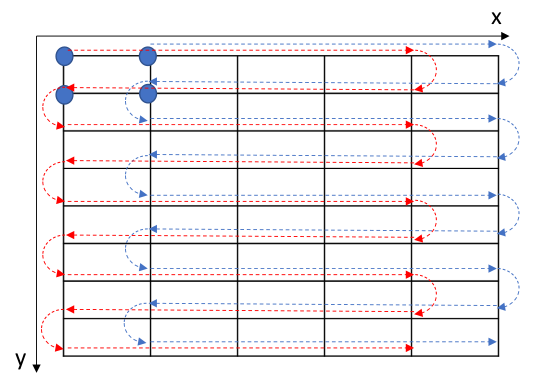
\includegraphics[width=3in]{figures/twoagentroute1.png}} 
 %\hspace{1in} 
  \subfigure[Routes of agents in the second line when $a=2$]{ 
    \label{fig:agentroute:b} %% label for second subfigure 
    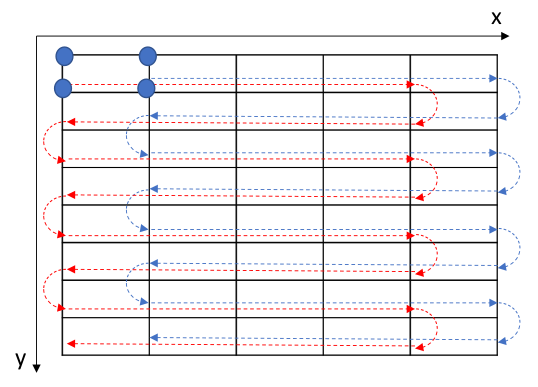
\includegraphics[width=3in]{figures/twoagentroute2.png}}
  \caption{Routes of agents when $a=2$} 
  \label{fig:twoagent2} %% label for entire figure 
\end{figure}
%\fi
when $a=3$, the routes of agents are shown as Fig\ref{fig:threeagent1}. 
\begin{figure} [H]
  \centering 
  \subfigure[Routes of agents in the first line when $a=3$]{ 
    \label{fig:agentroute:a} %% label for first subfigure 
    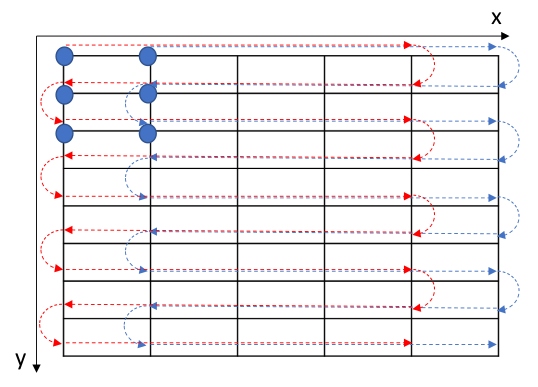
\includegraphics[width=3in]{figures/threeagentroute1.png}} 
  \hspace{1in} 
  \subfigure[Routes of agents in the second line when $a=3$]{ 
    \label{fig:agentroute:b} %% label for second subfigure 
    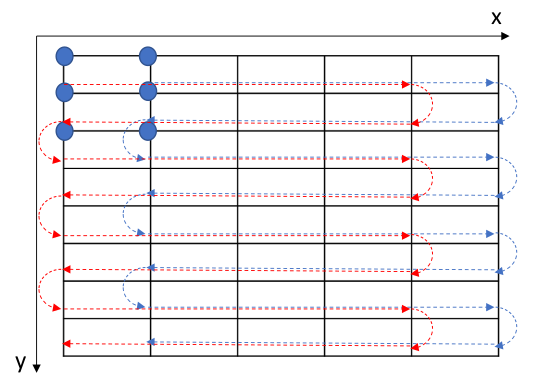
\includegraphics[width=3in]{figures/threeagentroute2.png}}
    \hspace{1in} 
    \subfigure[Routes of agents in the second line when $a=3$]{ 
    \label{fig:agentroute:c} %% label for second subfigure 
    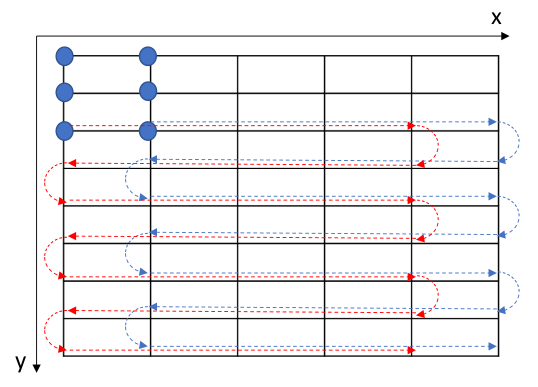
\includegraphics[width=3in]{figures/threeagentroute3.png}}
  \caption{Routes of agents when $a=3$} 
  \label{fig:threeagent1} %% label for entire figure 
\end{figure}
We can easily observe that some lines of the grid are traversed twice for the purpose of avoiding the explored nodes being contaminated (as shown in Fig \ref{fig:doubleline})
\begin{figure} [H]
  \centering 
  \subfigure[Lines that are double traversed when $a=2$]{ 
    \label{fig:agentroute:a} %% label for second subfigure 
    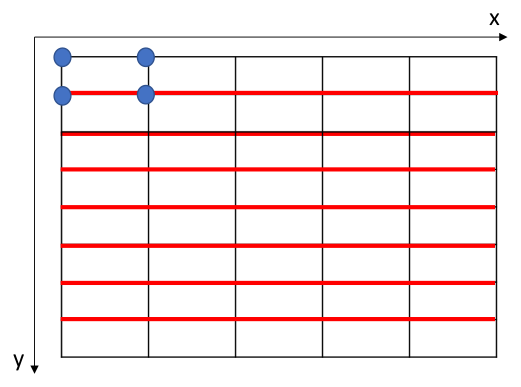
\includegraphics[width=3in]{figures/doubleline2.png}}
    %\hspace{1in} 
    \subfigure[Lines that are double traversed when $a=3$]{ 
    \label{fig:agentroute:b} %% label for second subfigure 
    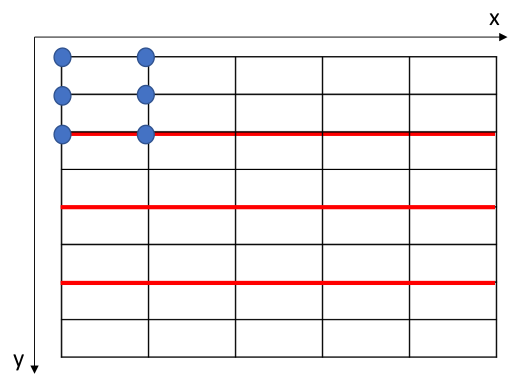
\includegraphics[width=3in]{figures/doubleline3.png}}
  \caption{Lines that are double traversed (marked with red lines)} 
  \label{fig:doubleline} %% label for entire figure 
\end{figure}
We can see that when the grid is fixed (so $d_1$ is fixed), the number of double traversed lines decrease as $a$ increases, which is easy to image. Let's denote by $r$ the number of lines that are double traversed, then $r=\left \lceil \frac{d_1-a}{a-1} \right \rceil$ where $d_1$ is the number of lines of the grid. Informally, $r$ reflect the time that we waste in the exploration phase, and we can reduce the wasted time by employing more agents. As we can see from the equation, when $a=d_1$, then $r=0$, which means if we employ $2d_1$ agents to explore the graph, none of the lines are traversed twice. \\
Now we discuss the strategy when we employ $2d_1$ agents, and this strategy can be easily modified to fit the situation where we employ less than $2d_1$ agents.\\
Initially, 2$d_1$ agents are placed at the first two columns at $T_0$ and we place another one agent at the top and bottom of the first column (we would describe their roles in the following part). More specifically, the coordinate of them are (1, $x_i$) and (2,$x_i$) where $1\leq x_i\leq d_1$. The agents residing in the first column are in the shadowing group while the agents residing in the second column are in the exploring group. If the BV resides in a node in the first column, then all of its clones are destroyed. If the BV resides in a node in the second column, then the elimination phase begins. It is obvious that if the BV do not reside in any node in the first column, then a agent in the exploring group should be destroyed when the BV is exposed.  Let's assume that the we starts at $T(t_0)$. Agents residing in nodes in the second column moves EAST at the beginning of $T(t_i)$, $i=0,1, \ldots ,d_2-1$. More precisely, node (x, y) move to (x+1, y) at the beginning of $T(t_i)$, $i=0,1, \dots , d_2-1$. Agents residing in the first column simply follow the node in the second column (see  Fig.\ref{fig:TShE}). When one of the node in the former column is destroyed by a BV, the second phase starts.
\begin{figure}[H]
  \centering  
  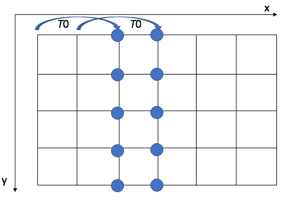
\includegraphics[width=2.5in]{figures/TShE.png}
  \caption{Agents move at time $T_0$. (The red node indicates that there are two agents residing there}\label{fig:TShE}
\end{figure}
\noindent{\bf Elimination Phase}\\
The elimination begins when one of the node in the former column is destroyed by a BV( let's say, at T($t_i$)). No matter where is the BV, there are always three agents residing on its north(if the BV is not in the first line), west and south (if the BV is not in the last line), so only one BV clone survives. In another word, only one node becomes BV node after the BV being triggered. Observe that in the parallel strategy, not all agents participate in the elimination phase automatically when the BV is explored because only those receive the clones of the original BV and those be notified by other agents can participate in the elimination phase. So in some situation, agents who receive the BV clone should notify other agents to participate in the elimination (case 1,2 and 3) and in one situation, we use the agent (the following agent) we take along the way to complete the elimination phase (case4). Let the node where the surviving clone resided be $(x, y)$ and its situation can be divided into four cases. Different routes of agents in the elimination phase are based on the location of the new formed BV.
\begin{itemize}
\item Case 1: When $2<x<d_1$, $1<y<d_2-1$ (a interior node becomes a new formed BV), then agents (let's say agents $a,b,c$) residing in node $(x-1, y+1)$, $(x-1, y-1)$ and $(x-2, y)$ receive a BV clone at T($t_i$), so that they know the location of the original BV and also the new formed BVs. After they receive the BV clone, these agents move EAST at T($t_i$+1) for one step (for example, to node $(x, y+1)$, $(x, y-1)$ and $(x-1, y)$ )and stop. Note that other agents including agents residing in node $(x-2, y+1)$ and $(x-2, y-1)$ (let's say agent d and e) at T($t_i$) do not know the existence of the BV so they keep moving EAST and arrive at nodes $(x, y+1)$, $(x, y-1)$ at the end of T($t_i+2$) when they meet agent $a$ and $b$ respectively. Agent $a$ and $b$ inform them of the location of the new form BV and the routes of agents $d$ and $e$ are as follow:\\
route of $d$: $(x, y+1)(at\ T(t_i+2){\rightarrow}(x+1,y+1)(at\ T(t_i+3){\rightarrow}(x+1,y)(at\ T(t_i+4)$.\\
route of $e$: $(x, y-1)(at\ T(t_i+2){\rightarrow}(x, y)(at\ T(t_i+5)$.
The routes of agents are showed in Fig.\ref{fig:caseone} where a blue node indicate that there is one agent residing here; a red node indicate that there are two agents residing here; a yellow node indicate that there are three agents residing here. 

%\iffalse
\begin{figure} [H]
  \centering 
  \subfigure[T($t_i$)]{ 
    \label{fig:caseone0:a} %% label for first subfigure 
    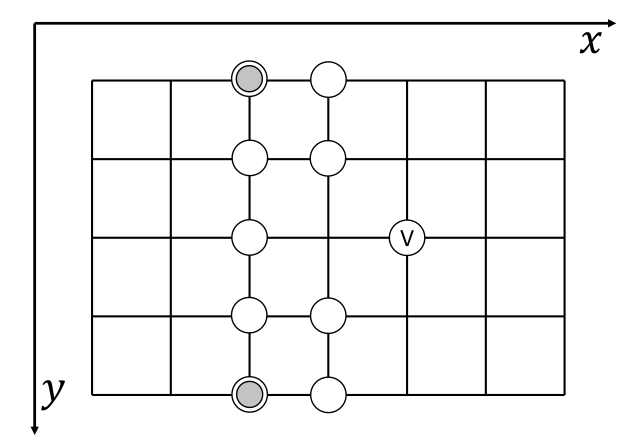
\includegraphics[width=2.5in]{figures/caseone0.png}} 
%  \hspace{1in} 
  \subfigure[T($t_i+1$)]{ 
    \label{fig:caseone1:b} %% label for second subfigure 
    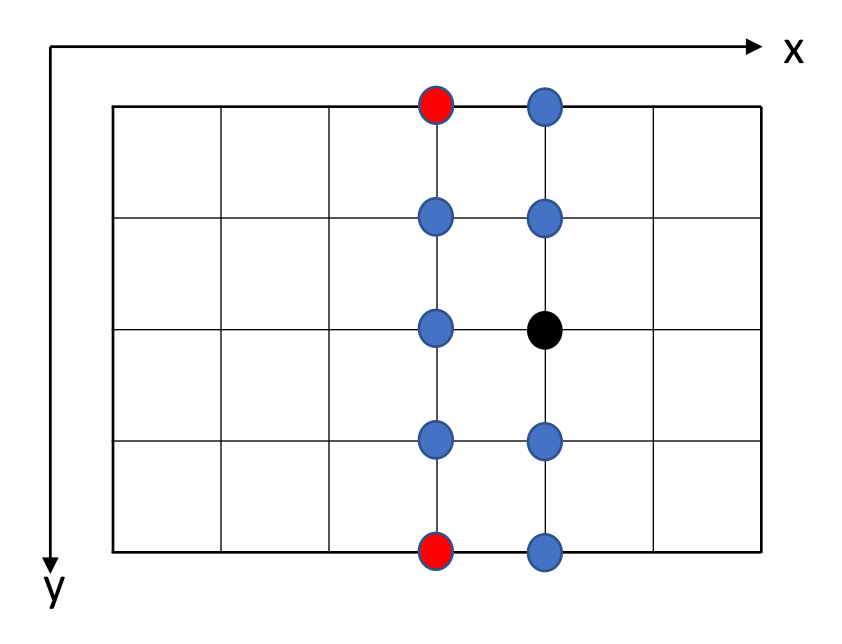
\includegraphics[width=2.5in]{figures/caseone1.png}}
    \hspace{1in} 
  \subfigure[T($t_i+2$)]{ 
    \label{fig:caseone2:c} %% label for second subfigure 
    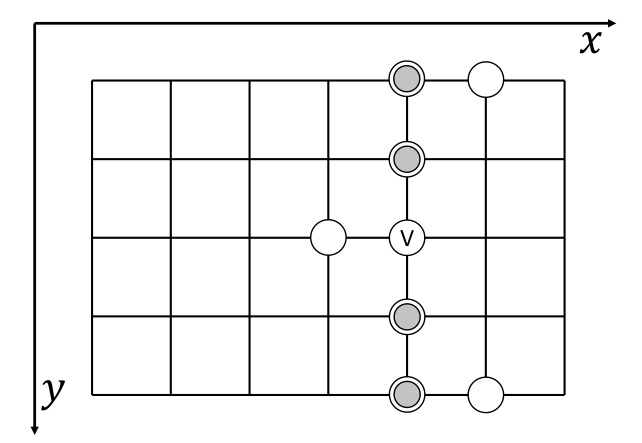
\includegraphics[width=2.5in]{figures/caseone2.png}}
%      \hspace{1in} 
  \subfigure[T($t_i+3$)]{ 
    \label{fig:caseone3:d} %% label for second subfigure 
    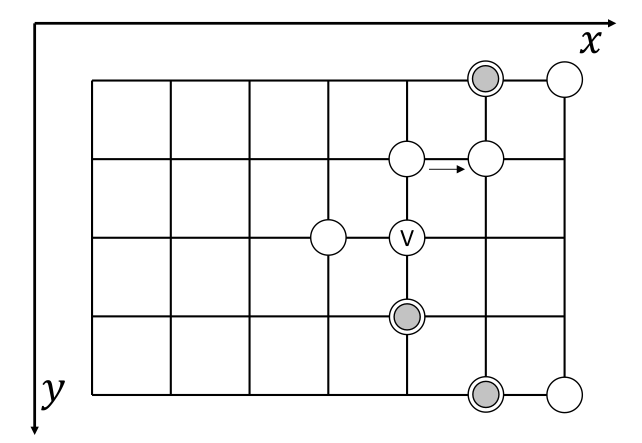
\includegraphics[width=2.5in]{figures/caseone3.png}}
      \hspace{1in} 
  \subfigure[T($t_i+4$)]{ 
    \label{fig:caseone4:e} %% label for second subfigure 
    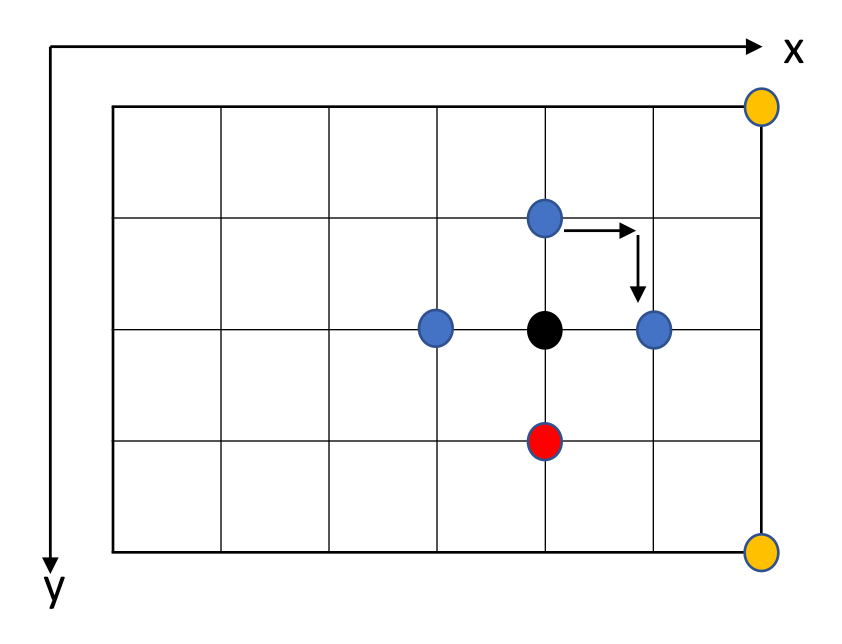
\includegraphics[width=2.5in]{figures/caseone4.png}}
     \subfigure[T($t_i+5$)]{ 
    \label{fig:caseone5:e} %% label for second subfigure 
    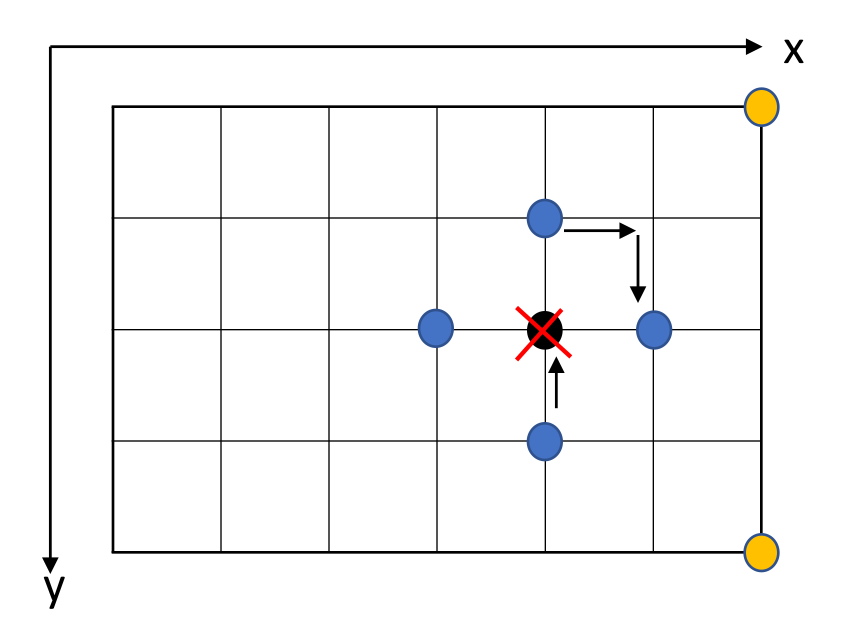
\includegraphics[width=2.5in]{figures/caseone5.png}}
  \caption{Arrangement of agents in elimination phase when the new formed BV resides in a interior node} 
  \label{fig:caseone} %% label for entire figure 
\end{figure}
%\fi

\item Case 2: When $x=d_1$, $2<y<d_2-1$ (a border node becomes a new formed BV), then agents (let's say agents $a,b,c$) residing in node $(x-1, y+1)$, $(x-1, y-1)$ and $(x-2, y)$ receive a BV clone at T($t_i$). As above, they move EAST for one step and stop. Agents residing in nodes $(x-2, y+1)$ and $(x-2, y-1)$ (let's say agents $a,b$) at T($t_i$) have no knowledge of the BV, so they keep moving and arrive at nodes $(x, y+1)$ and $(x, y-1)$ at T($t_i$+2) when they are informed of the location of the new formed BV. One of agents $a$ and $b$ should move to the new formed BV to decontaminate it while the other one stop moving at T($t_i$+3). In order to avoid conflict, we always employ the agent $a$ to move to the new formed BV. (see Fig\ref{fig:casetwo})
\begin{figure} [H]
  \centering 
  \subfigure[$T(t_i)$]{ 
    \label{fig:casetwo0:a} %% label for first subfigure 
    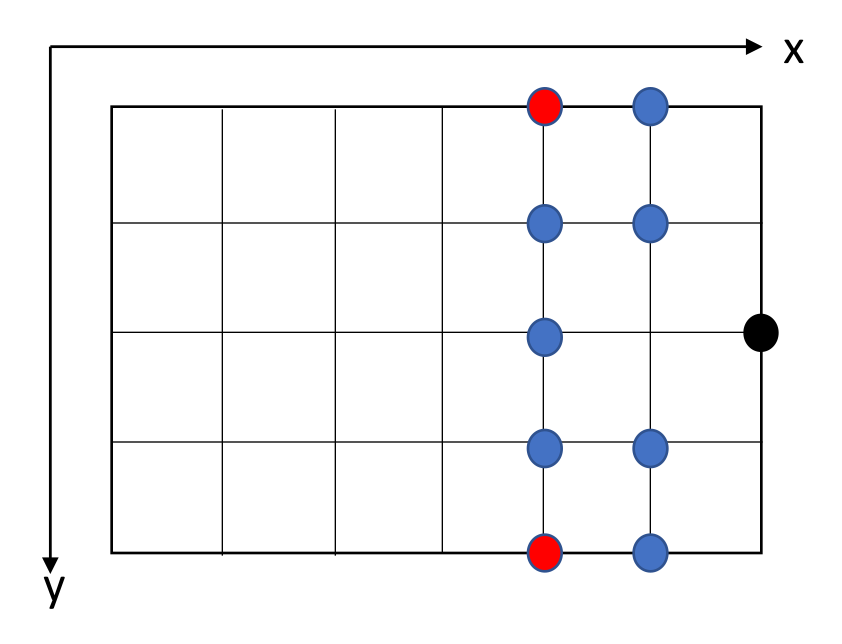
\includegraphics[width=2.5in]{figures/casetwo0.png}} 
%  \hspace{1in} 
  \subfigure[$T(t_i+1)$]{ 
    \label{fig:casetwo1:b} %% label for second subfigure 
    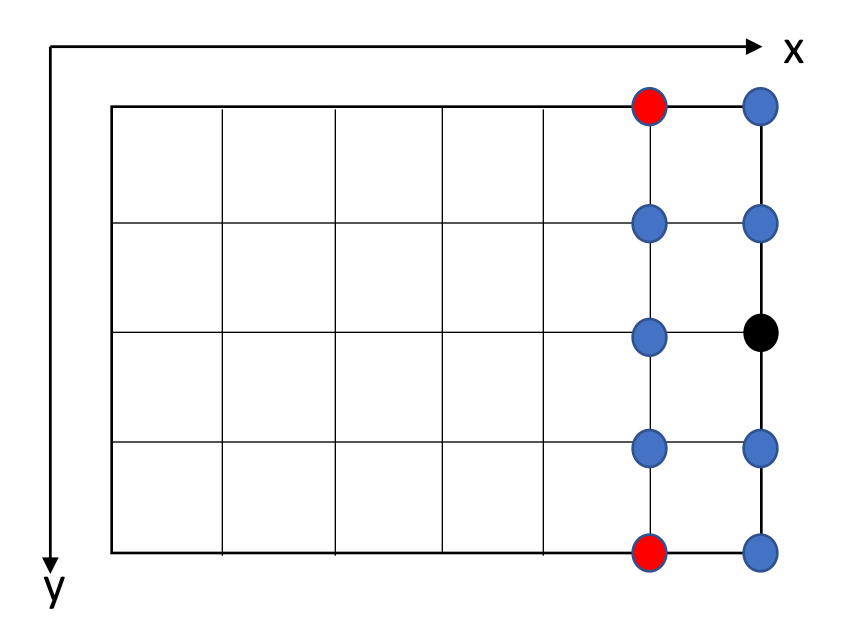
\includegraphics[width=2.5in]{figures/casetwo1.png}}
    \hspace{1in} 
  \subfigure[$T(t_i)+2$]{ 
    \label{fig:casetwo2:c} %% label for second subfigure 
    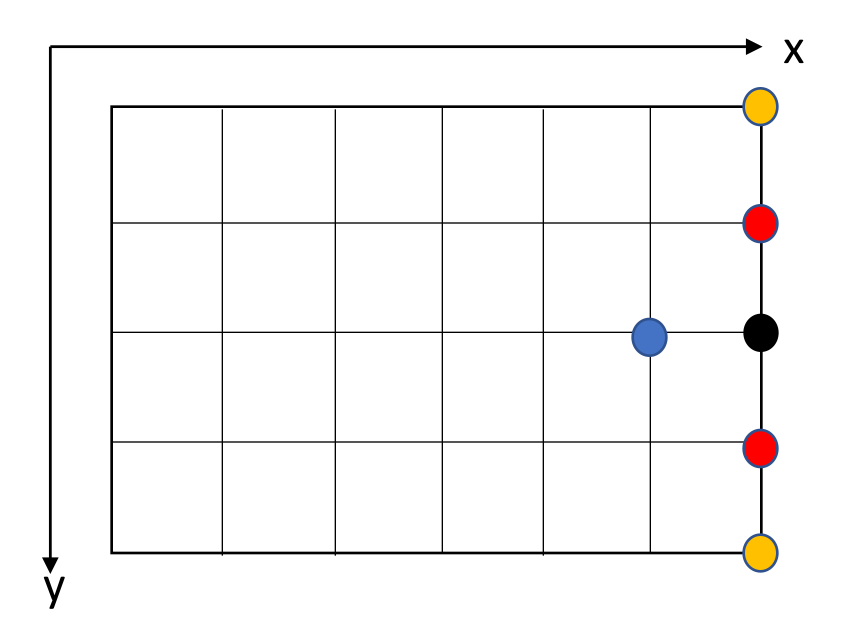
\includegraphics[width=2.5in]{figures/casetwo2.png}}
%      \hspace{1in} 
\subfigure[$T(t_i)+3$]{ 
    \label{fig:casetwo3:d} %% label for second subfigure 
    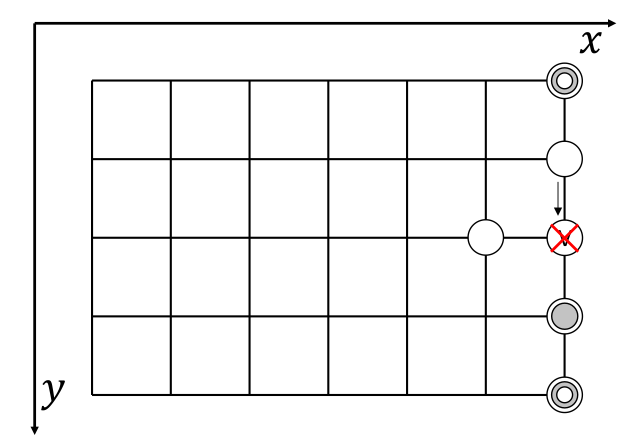
\includegraphics[width=2.5in]{figures/casetwo3.png}}
    \caption{Arrangement of agents in elimination phase when the new formed BV resides in a border node (when $x=d_1$)} 
  \label{fig:casetwo} %% label for entire figure 
\end{figure}

\item Case 3: When $2<x<d_1$, $y=1$ or $y=d_2-1$ (a border node becomes a new formed BV). For convenience, we only discuss the situation when $y=1$(the solution can be easily modified to fit the scenario when $y=d_2-1$). In this case, agents residing in nodes $(x-1, y+1)$ and $(x-2, y)$ (let's say agents a,b,c(the following agent)) receive a BV clone at T($t_i$). Agents $a$, $b$ and $c$ move EAST for one step and arrive at node $(x, y+1)$ and node $(x-1, y)$ at T($t_i+1$). Agent in node $(x-2, y+1)$ does not know the existence of the BV, so it keep 
%\iffalse
\begin{figure} [H]
  \centering 
  \subfigure[T($t_i$)]{ 
    \label{fig:casethree0:a} %% label for first subfigure 
    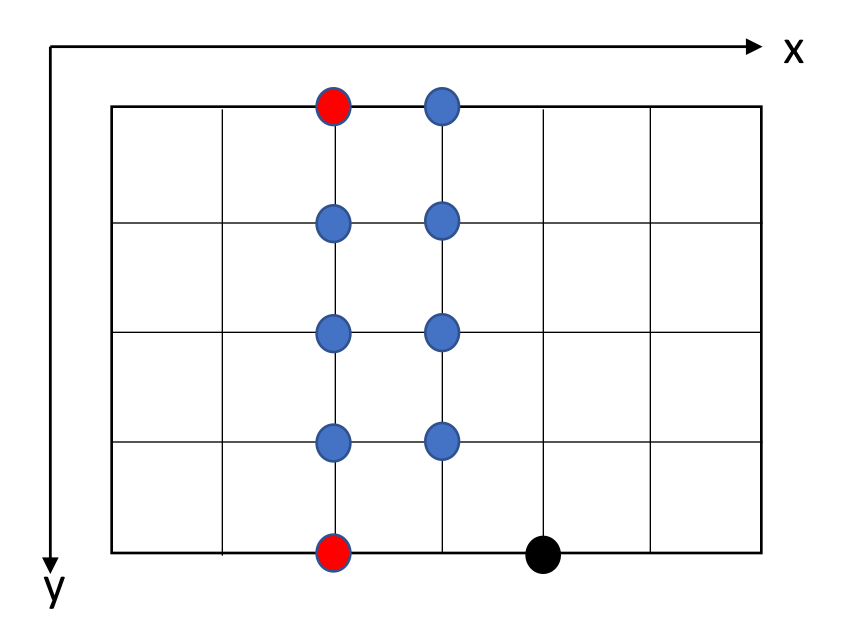
\includegraphics[width=2.5in]{figures/casethree0.png}} 
%  \hspace{1in} 
  \subfigure[T($t_i+1$)]{ 
    \label{fig:casethree1:b} %% label for second subfigure 
    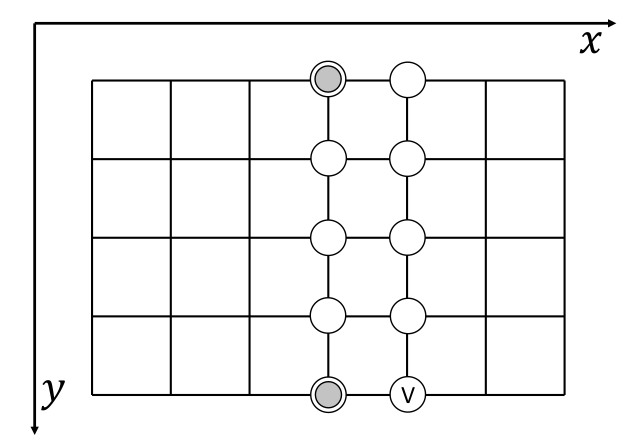
\includegraphics[width=2.5in]{figures/casethree1.png}}
    \hspace{1in} 
  \subfigure[T($t_i+2$)]{ 
    \label{fig:casethree2:c} %% label for second subfigure 
    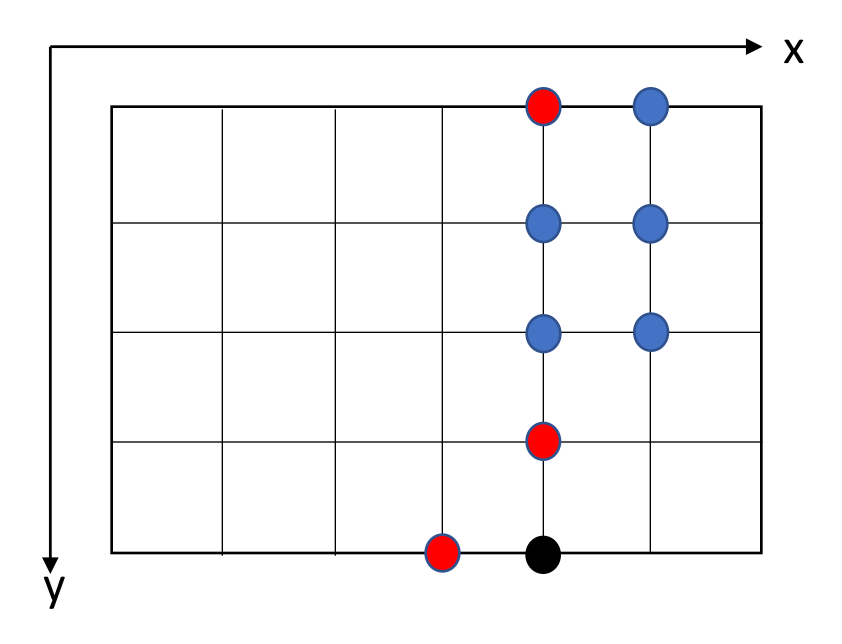
\includegraphics[width=2.5in]{figures/casethree2.png}}
%      \hspace{1in} 
  \subfigure[T($t_i+3$)]{ 
    \label{fig:casethree3:d} %% label for second subfigure 
    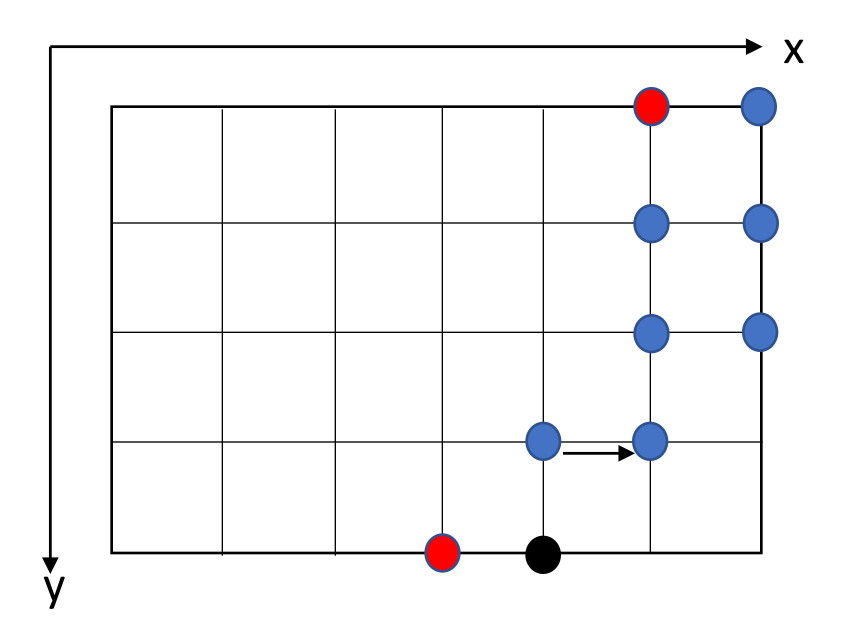
\includegraphics[width=2.5in]{figures/casethree3.png}}
      \hspace{1in} 
  \subfigure[T($t_i+4$)]{ 
    \label{fig:casethree4:e} %% label for second subfigure 
    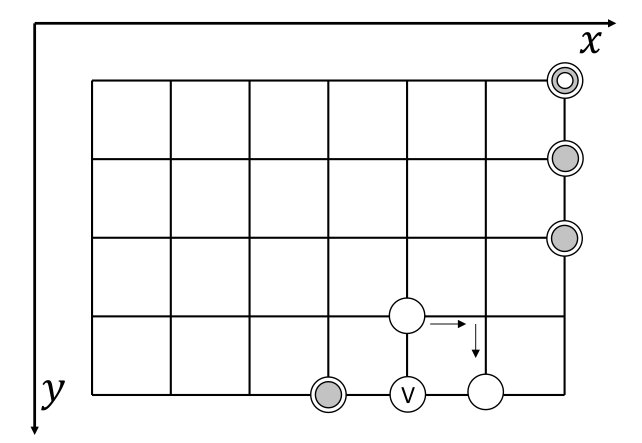
\includegraphics[width=2.5in]{figures/casethree4.png}}
     \subfigure[T($t_i+5$)]{ 
    \label{fig:casethree5:e} %% label for second subfigure 
    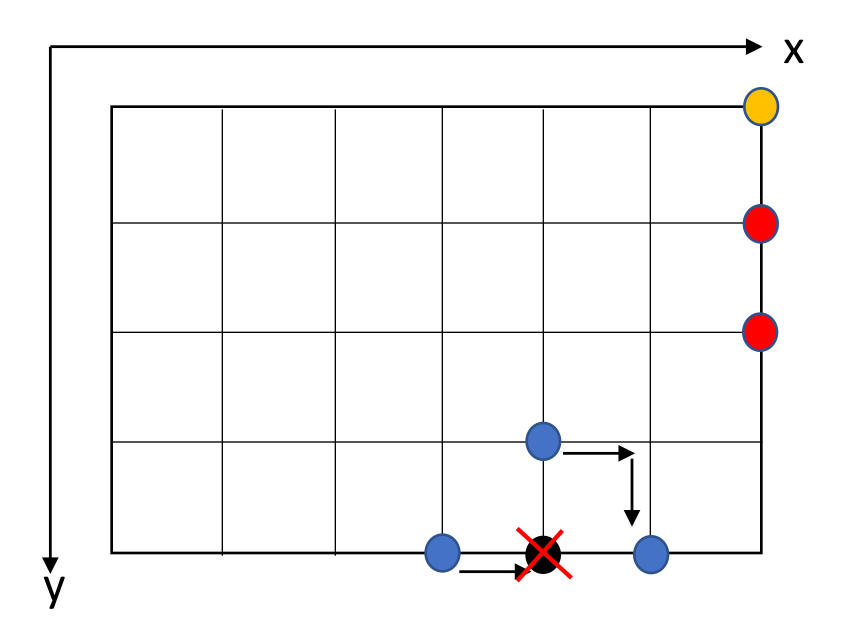
\includegraphics[width=2.5in]{figures/casethree5.png}}
  \caption{Arrangement of agents in elimination phase when the new formed BV resides in a interior node} 
  \label{fig:casethree} %% label for entire figure 
\end{figure}
%\fi

\item Case 4: When $x=d_1$ and $y=1$ or $y=d_2-1$ (a corner node becomes a new formed BV). For convenience, we only discuss the situation when $y=1$. In this case, agents residing in node $(x-1, y+1)$ and $(x-2, y)$ (let's say agents a,b) receive a BV clone at T(2$x_i$). Both of them keep moving for one step and arrive at nodes $(x, y+1)$ and $(x-1, y)$ at T$(2(x_i+1))$.
\begin{figure} [H]
  \centering 
  \subfigure[$T(2x_i+1)$]{ 
    \label{fig:subfigmesh4:a} %% label for first subfigure 
    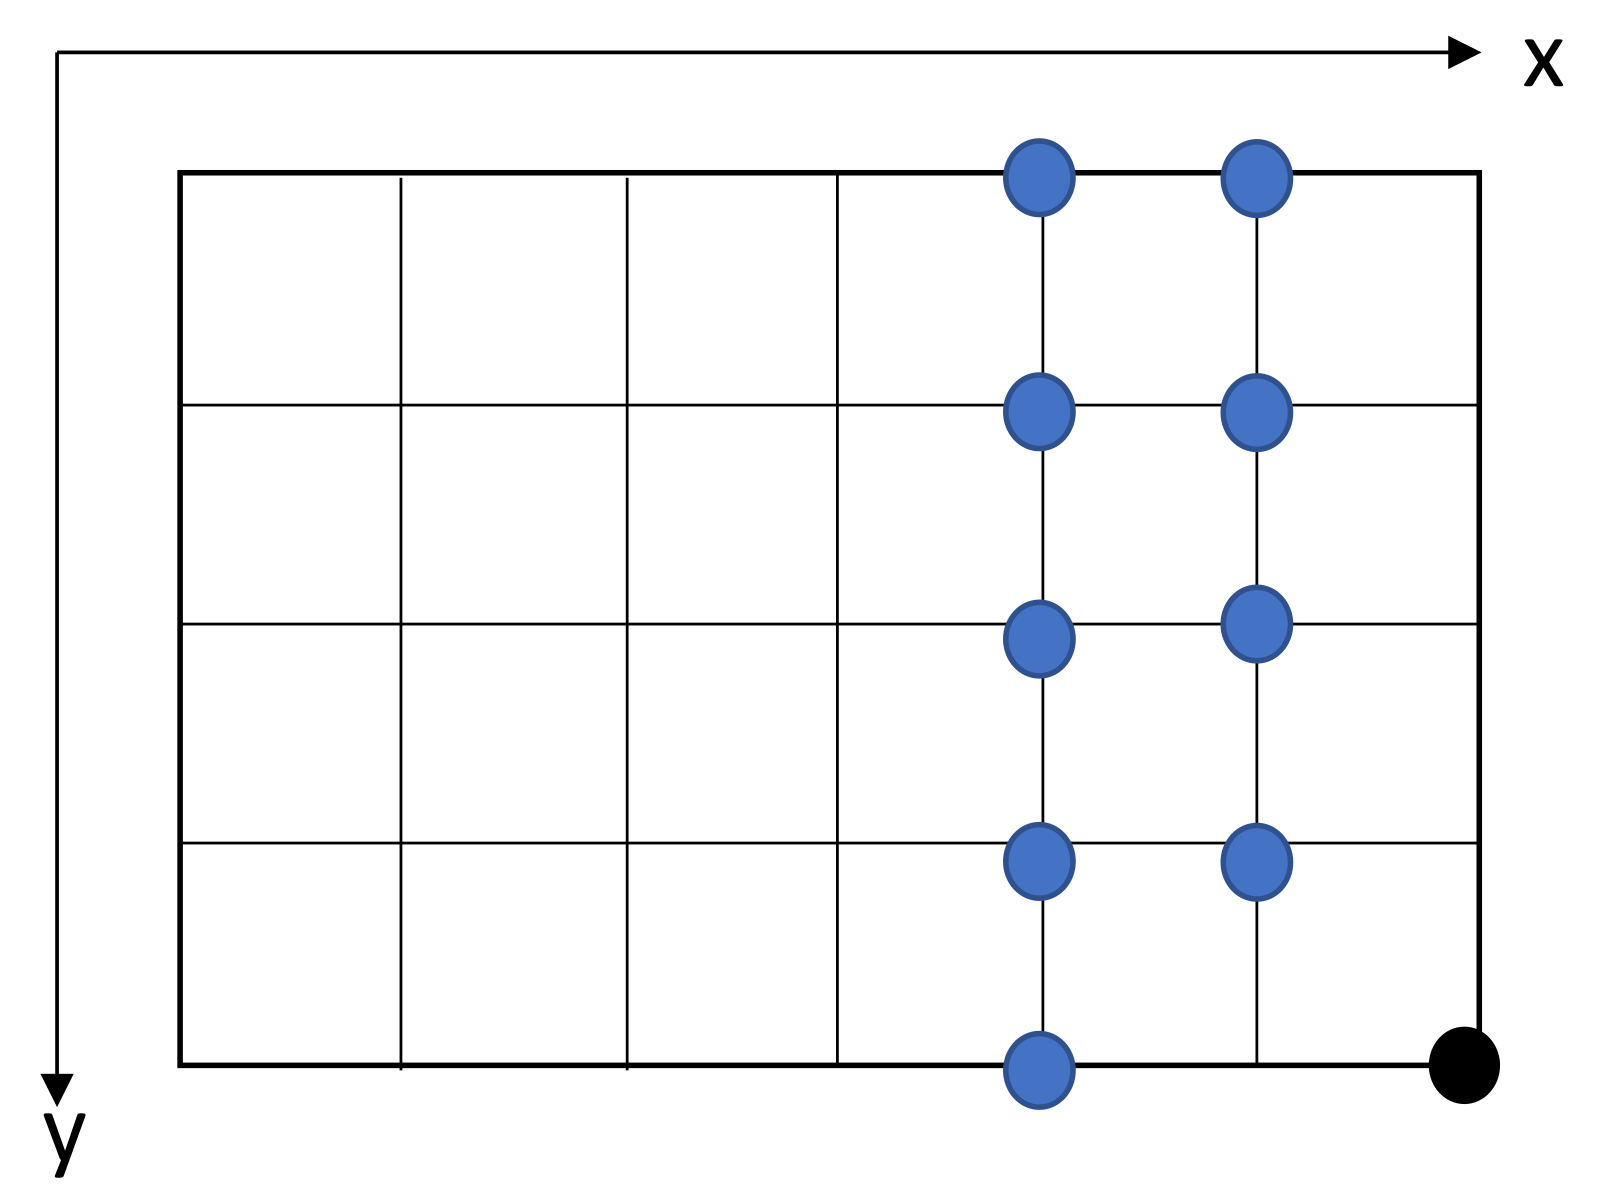
\includegraphics[width=2.5in]{figures/meshcorner1.png}} 
% \hspace{1in} 
  \subfigure[$T(2(x_i+1))$]{ 
    \label{fig:subfigmesh4:b} %% label for second subfigure 
    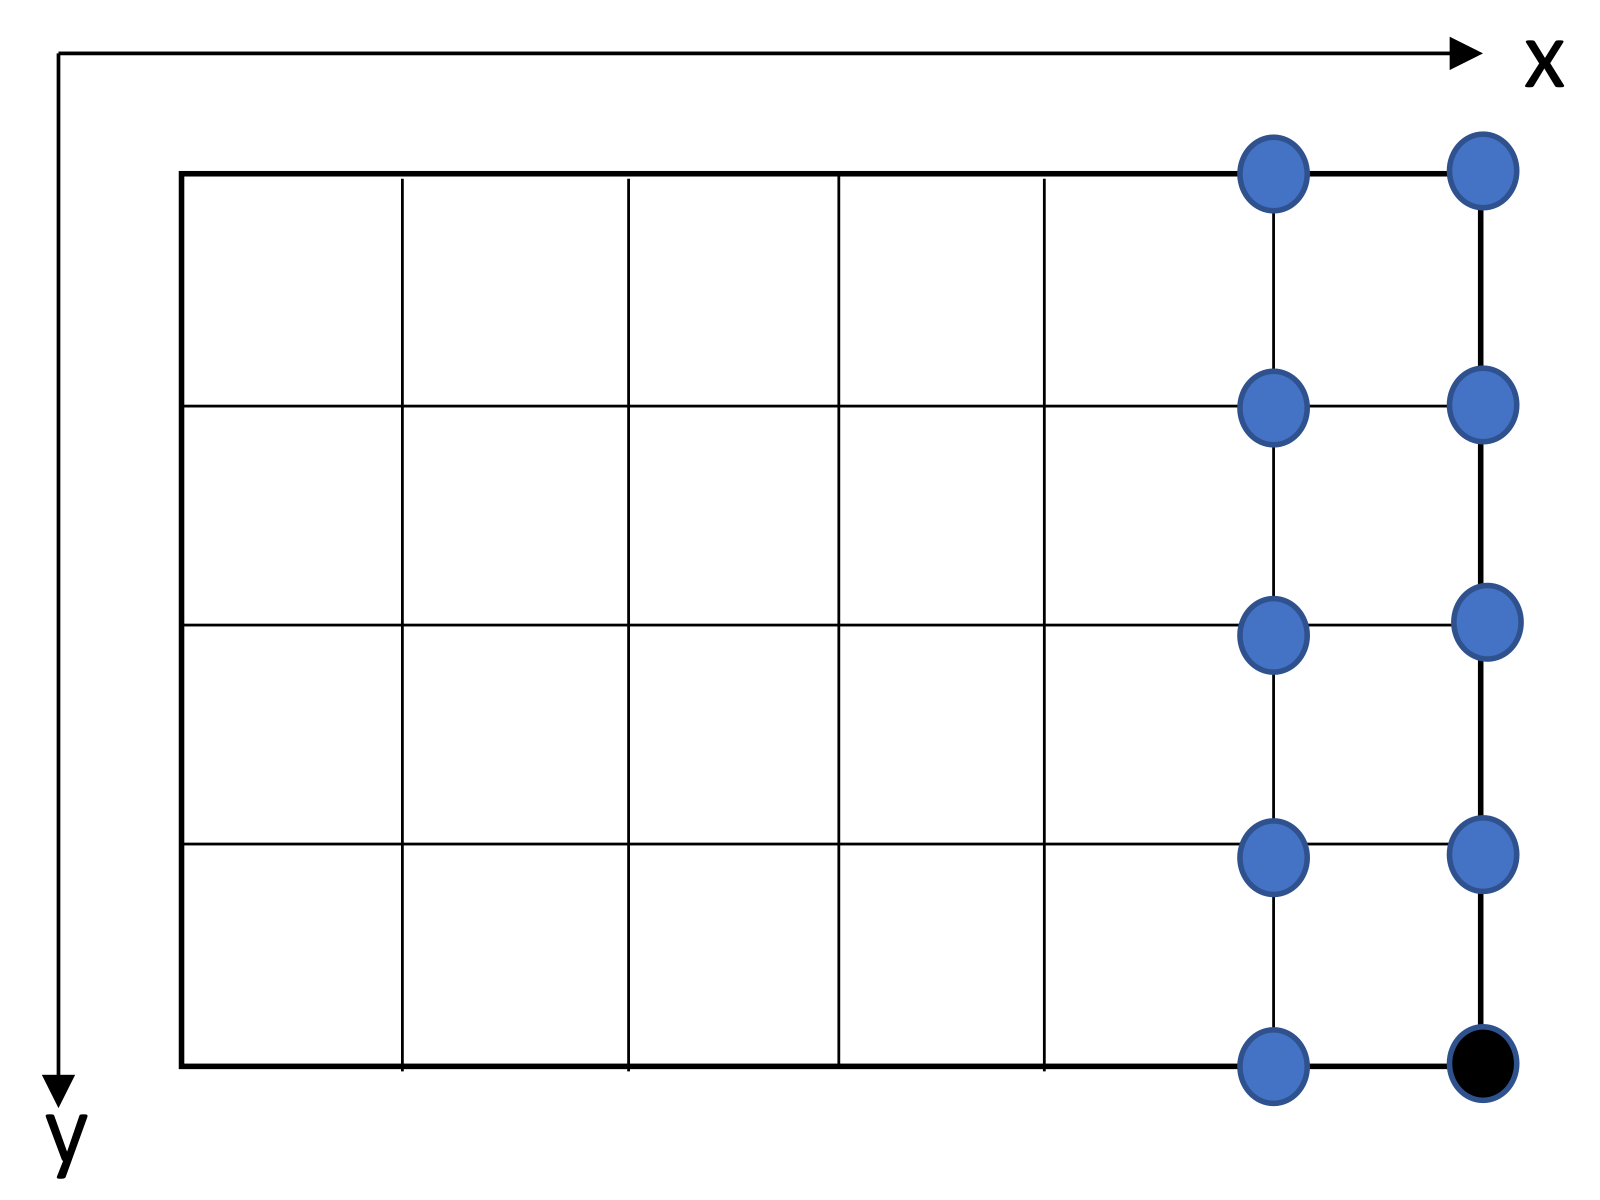
\includegraphics[width=2.5in]{figures/meshcorner2.png}}
 \hspace{1in} 
  \subfigure[$T(2(x_i+2))$]{ 
    \label{fig:subfigmesh4:c} %% label for second subfigure 
    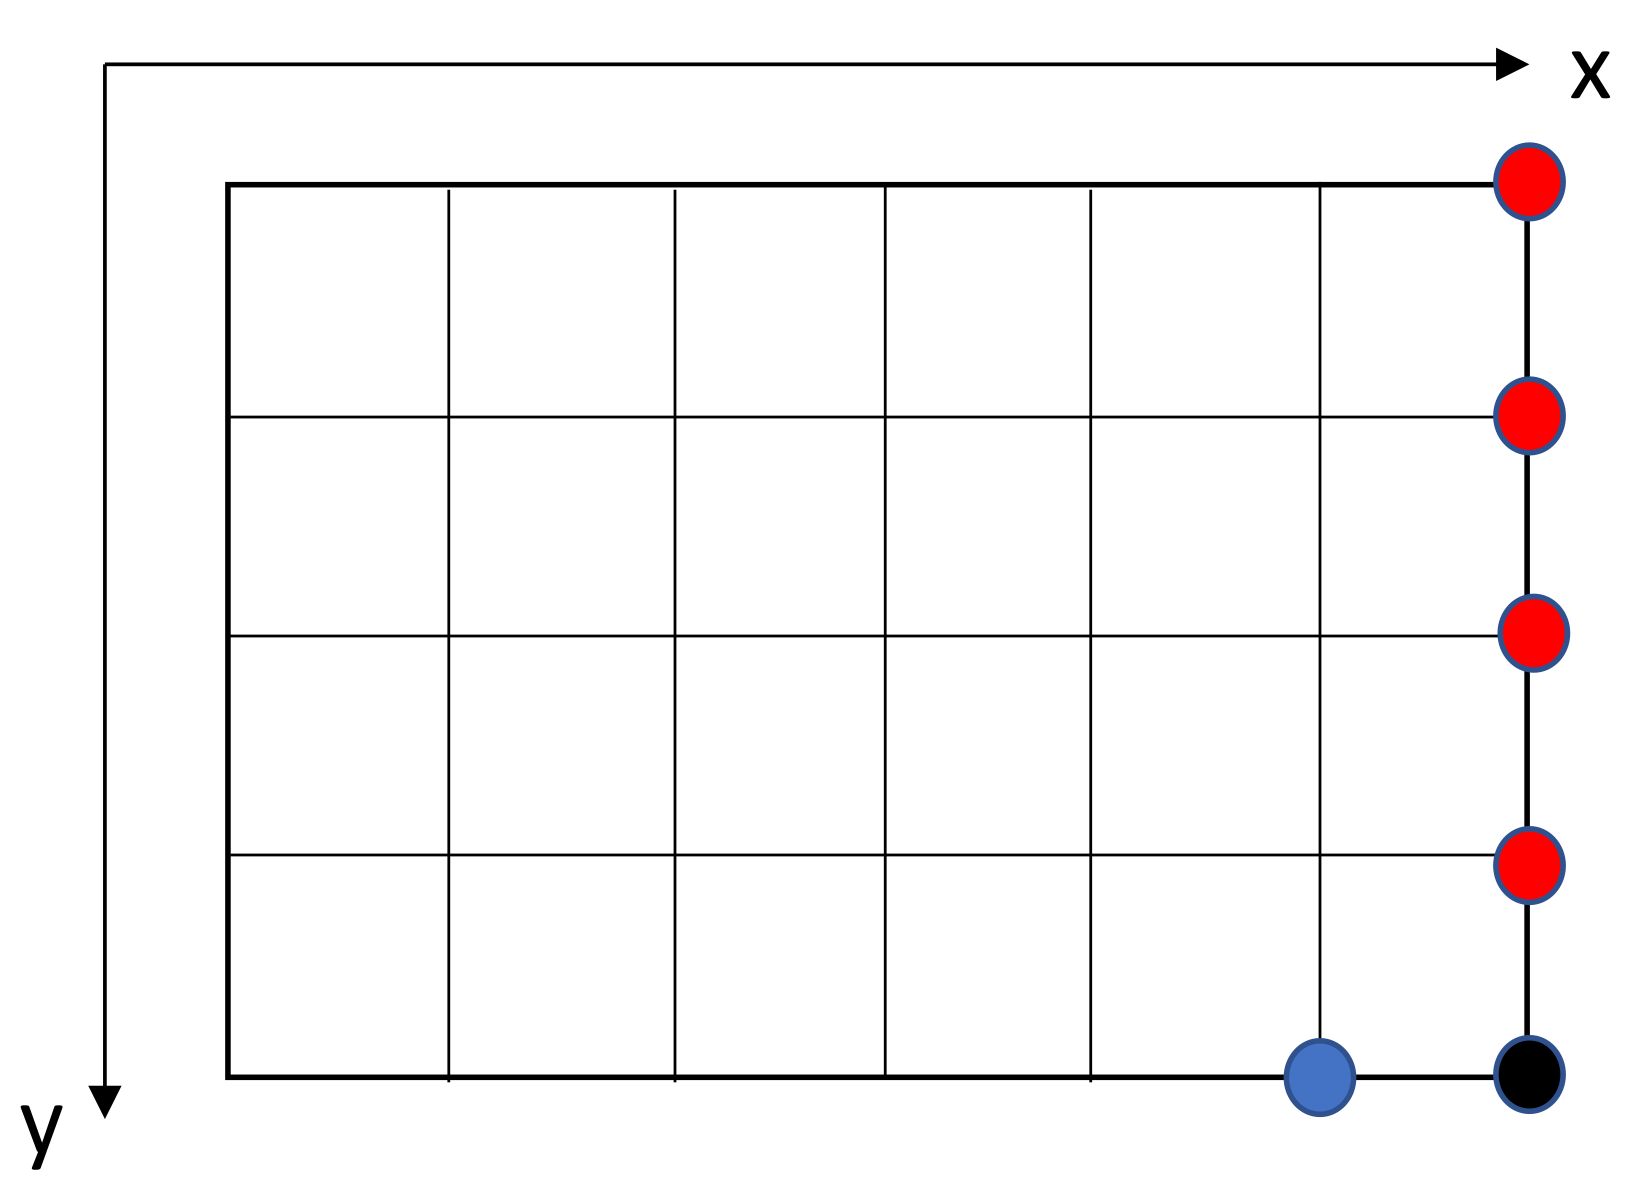
\includegraphics[width=2.5in]{figures/meshcorner3.png}}
%      \hspace{1in} 
\subfigure[$T(2(x_i+2)+1)$]{ 
    \label{fig:subfigmesh4:d} %% label for second subfigure 
    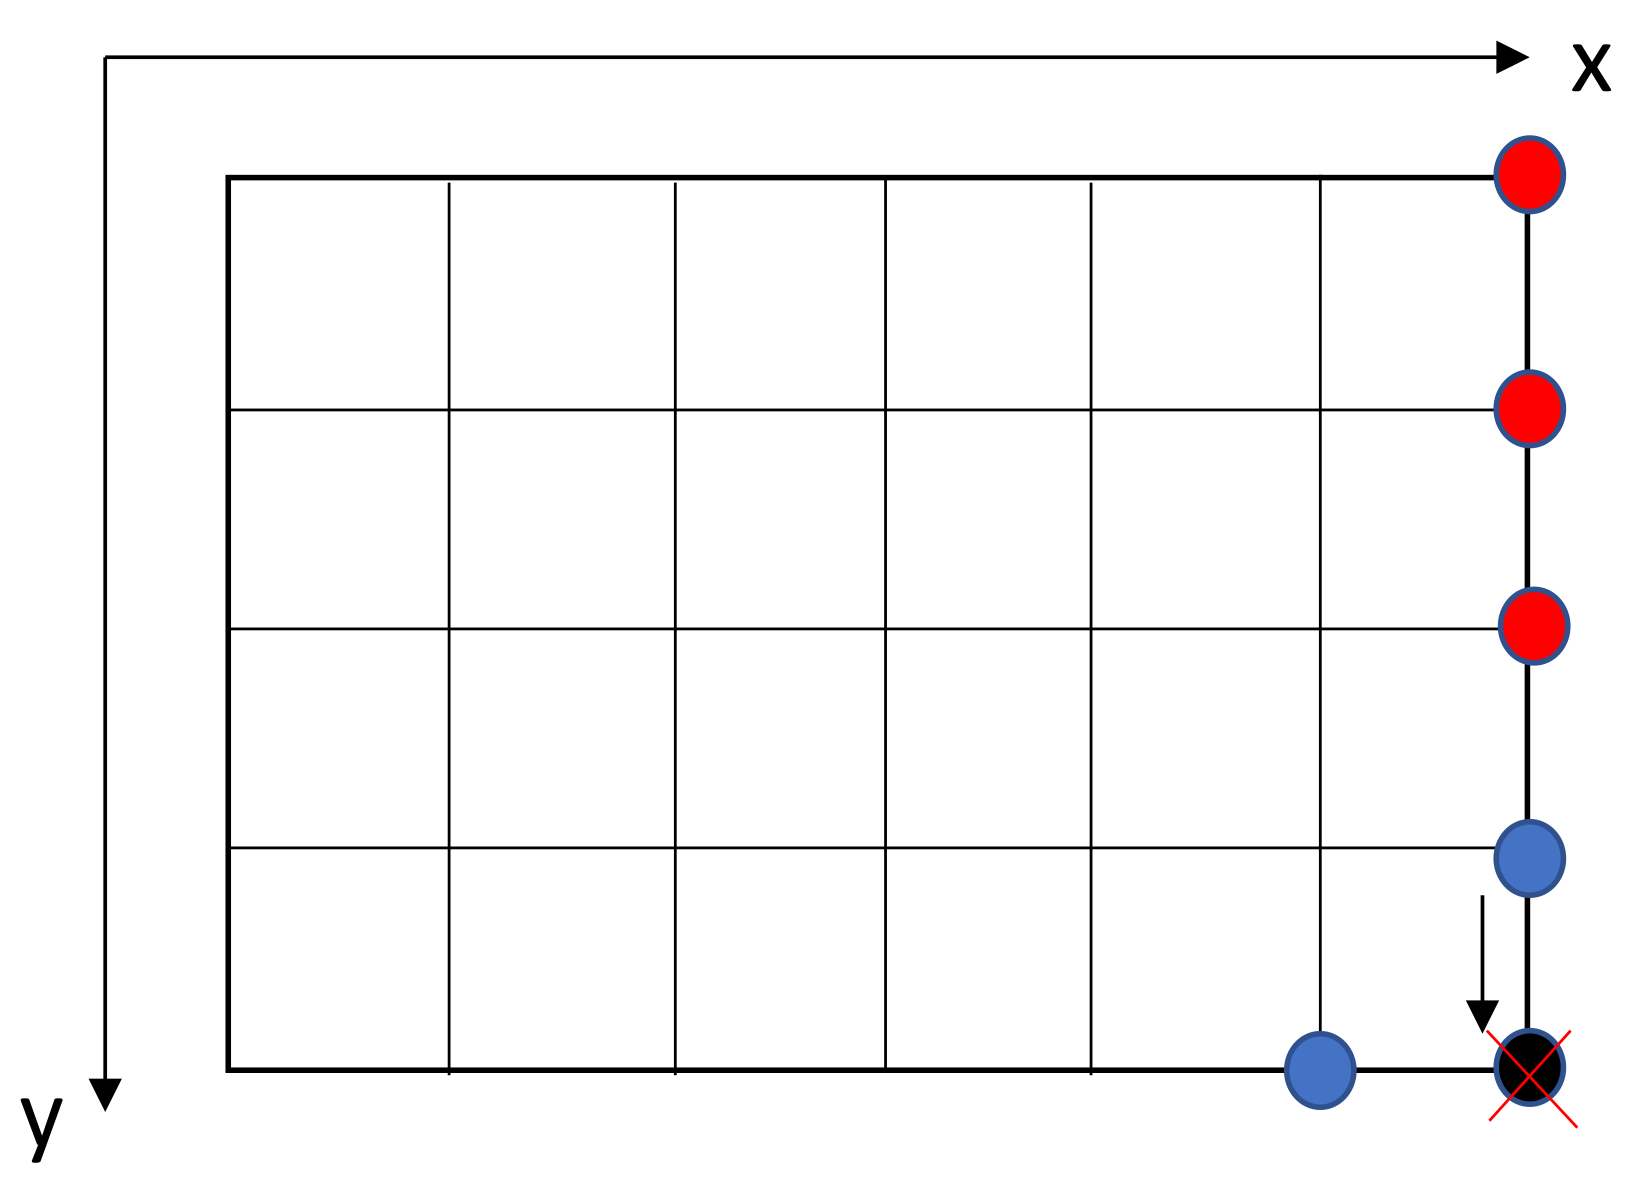
\includegraphics[width=2.5in]{figures/meshcorner4.png}}
    \caption{Arrangement of agents in elimination phase when the new formed BV resides in a corner (when $x=d_1$ and $y=1$ or $y=d_2-1$)} 
  \label{fig:subfigmesh4} %% label for entire figure 
\end{figure}
\end{itemize}

\noindent{\bf Analysis and Comparing}
\begin{theorem}
Mesh contamination algorithm performs a decontamination of a mesh (size of $n=d_1\times d_2(d_1>2,d_2>2)$ using $k=2(\sqrt{n}+1)$ agents and at most 1 casualties.
\end{theorem}
\begin{proof}
Let $v=(x, y)$ be the node containing the BV. When one of the agent in the exploring group moves to $v$, it will be destroyed and the BV will move to all neighbours of $v$. If $x=1$, then the neighbours $(x, y+1)$, $(x, y-1)$ and $(x+1, y)$ are protected by agents and neighbour $(x-1, y)$ actually does not exist; if $x>1$, then neighbours $(x, y+1)$, $(x, y-1)$ and $(x-1, y)$ are protected by agents. So when the clones of BV moves to the neighbours of $v$, those contain a agent will not be infected by the BV clone; this means that the BV can safely move only to the unexplored neighbours of $v$, of which are at most one. In other words, after $v$ is explored, at most one BV node are formed. According to our elimination strategy, the new formed BV node can be surrounded and destroyed using at most five agents: one to enter a BV and four to protect the neighbours. Since we have one new formed BV, the number of agents participating in the elimination phase is at most five. In addition to the agent destroyed by the original BV, the number of agent needed to complete the elimination phase is at least six. Since we employ $k=2d_1$ ($d_1\geq 3$) which means at the beginning we have at least six agents, so $2d_1$ agents are enough for the decontamination algorithm.
\end{proof}
Let us now consider the number of movements.
\begin{theorem}
Parallel mesh decontamination algorithm performs a BV decontamination of a mesh of size n with at most $2n-\sqrt{n}+O(1)$ movements in time at most $\sqrt{n}+11$.
\end{theorem}
\begin{proof}
Let $v=(x, y)$ be the BV node, and let the size of the grid be $n=d_1\times d_2$. Let us first consider the number of movements performed during the shadowed exploration. Since all the agents simply move EAST at the beginning of T(2n) ($n=0,1, \dots , d_2-1$), the travelling distance is $x$ for agents in the exploring group ({em EA}) and $x-1$ for agents in the shadowing group({em SA}). We have $d_1$ {\em EAs} and $d_1$ {\em SAs}, then we have an overall cost of at most $d_1\times (2x-1)$ movements for this phase.
Consider now the number of movements performed for Surrounding and Elimination. In this part, we only compute the movements of the agents who participate in the Surrounding and Elimination. More specifically, we simply ignore the movements of the agents who do not know the existence of the BV in the whole process. As we discuss in the Elimination phase, when the new formed BV is located in a interior node, ten movements are needed in this phase; when the new formed BV is located in a border node (let' s say $(a, b)$), then eight movements are needed when $a=d_1, 2< b <d_2-1$ and eleven movements are needed when $2< a <d_1,b=1 or b=d_2-1$; when the new formed BV is located in a corner node, then five movements are needed in this phase. Hence $O(1)$ movements are performed in this phase.
In total we have that the number of movements is at most $d_1 \times(2x-1)+O(1)\leq \sqrt{n}\times(2\sqrt{n}-1)+O(1)$, which is $2n-\sqrt{n}+O(1)$.\\
As for the time complexity. The time required for the exploration phase is equal to the number of movements of EA, which is $d_1$; the time required for the surrounding and elimination phase is at most eleven. So in total the parallel mesh decontamination algorithm terminate in time at most $\sqrt{n}+11$. 
\end{proof}

Now we make some comparison between our strategy and the sequential strategy.

\begin{table} [hbtp]
\caption{Comparision between PBVD-2G and BVD-2G}
\label{table:ComparisionPBVD-2GandBVD-2G}
\centering
\tabulinesep=2mm
\begin{tabu} to 140 mm {|X[6,c]|X[4,l]|X[4,l]|X[4,l]|X[4,l]|} \hline 
%\begin{tabular}{|c|l|} \hline 
& The number of agent & The time cost & The number of movement & The casualties \\ \hline
{\em PBVD-2G}   & $2\sqrt{n}$   & $\sqrt{n}+11$ & $2n-\sqrt{n}+O(1)$   & 1        \\ \hline
{\em BVD-2G} & 7    & $3n$          & $9n+O(1)$     & 3              \\ \hline
\end{tabu}
%\end{tabular}
\end{table}

\subsection{Multi-Dimensional Grid}
Let $M$ be a q-dimensional grid of size $d_1\times\ldots\times d_q$ and let each node of $M$ be denoted by its coordinates $(x_1,\ldots,x_q)$, $1\leq x_i\leq d_q$. The algorithm, called {\em PBVD-qG}, follows a general strategy similar to the one described in Section 4.2.1: a safe exploration with shadowing, followed by a surrounding and elimination phase. Our general idea is that: (1) Transform the PBVD-qG problem into a BVD-qG problem (2) Use the BVD-qG strategy to solve the transformed problem. We want to solve the problem parallelly, so for convenience, if we use "q-dimensional" agent group, we use $d_1\times \ldots \times d_p$ agents and they are organized in a $d_1\times \ldots \times d_p$ grid. 
In \cite{Cai}, the multi-dimensional grid is partitioned into $d_1\times \ldots d_(q-2)$ 2-dimensional grids of size $d_(q-1) \times d_q$. Each of these grids is explored using the BVD-2G: after traversing a grid in a snake-like fashion column by column, the agent returns to the starting point and from that starting point, it proceeds to another grid with a neighbouring starting point. In our strategy PBVD-qG, we use the similar exploring routes as that in BVD-G which is the snake-like route. Additionally, we use the idea of dimensionality reduction. Informally, when we solve the parallel contamination problem in q-dimensional grid using ``p-dimensional" agent group, we can view the ``p-dimensional" agent group as one ``large agent" and view the q-dimensional grid as a ``(q-p)-dimensional grid. So when we increase the number of the agents (for example, increase the ``p"), then actually we decrease the dimension of the grid we want to explore. For example, if we want to solve the BVD problem in a 4-dimensional grid (say in a $d_1 \times\ d_2 \times d_3\times d_4$ grid) using the PBVD-2G and we use $d_1$ agents to explore it. The problem can be viewed as using one ``large" agent to explore a $d_2\times d_3\times d_4$ grid. If we use $d_1\times d_2$ agents to explore it, then the problem can be viewed as using one ``large" agent to explore a $d_3 \times d_4$ grid. We can choose the dimension of the agent group at the beginning and Fig\ref{fig:4dimensional} shows how can we view a higher dimensional grid as a lower dimensional grid. 

\begin{figure} [H]
  \centering 
  \subfigure[The arrangement of agents on a 4-dimensional grid]{ 
    \label{fig:4dimensional1:a} %% label for first subfigure 
    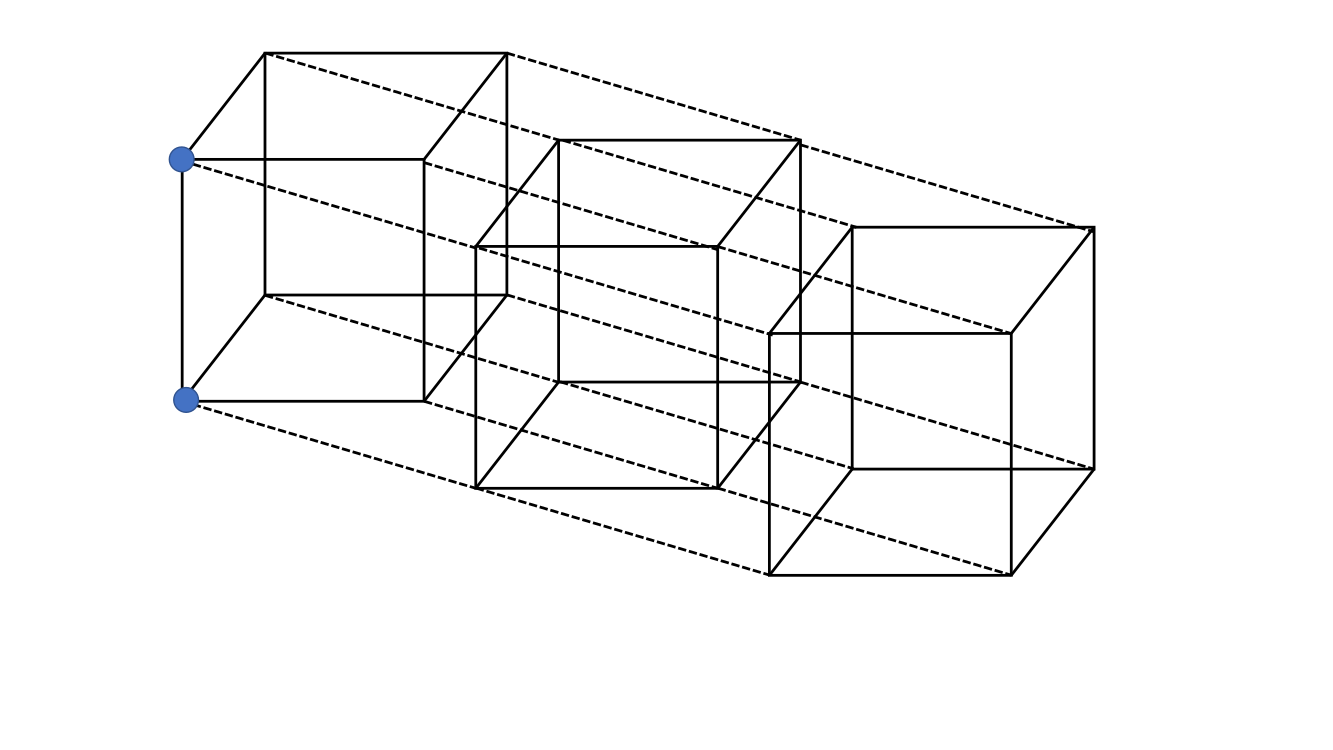
\includegraphics[width=2.8in]{figures/4dimensional1.png}} 
% \hspace{1in} 
  \subfigure[When we view the ``one dimensional" agent as a large agent and the grid can be view as a three dimensional grid]{ 
    \label{fig:4dimensional2:b} %% label for second subfigure 
    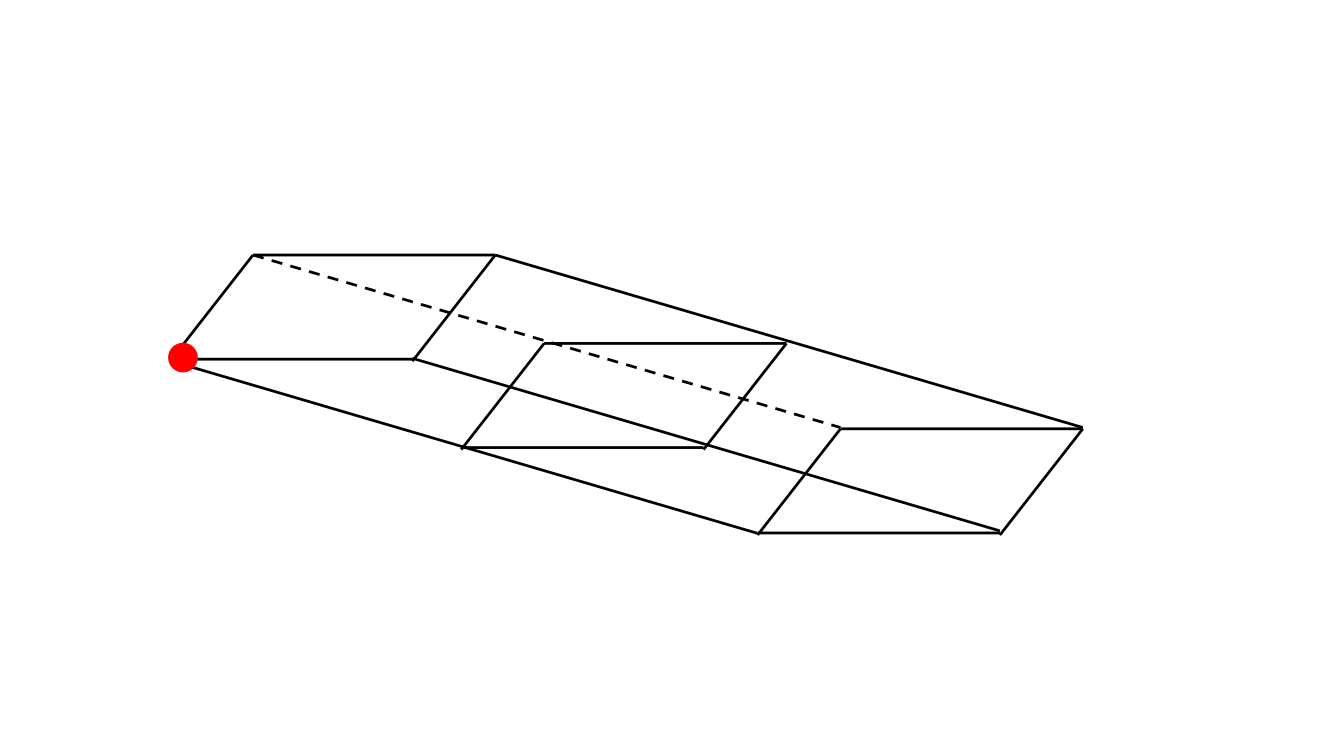
\includegraphics[width=2.8in]{figures/4dimensional2.png}}
 \hspace{1in} 
  \subfigure[The arrangement of agents on a 4-dimensional grid]{ 
    \label{fig:4dimensional3:c} %% label for second subfigure 
    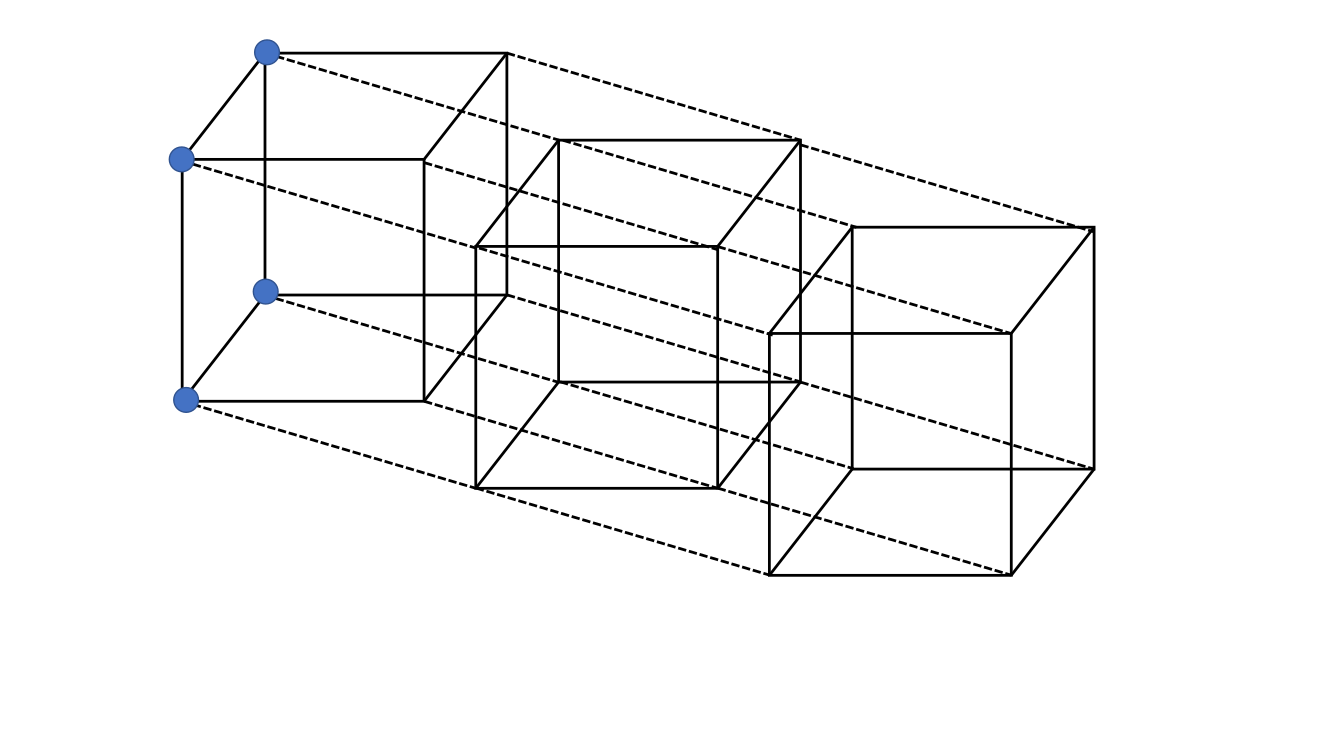
\includegraphics[width=2.8in]{figures/4dimensional3.png}}
%\hspace{1in} 
\subfigure[When we view the ``two dimensional" agent as a large agent and the grid can be view as a two dimensional grid]{ 
    \label{fig:4dimensional4:d} %% label for second subfigure 
    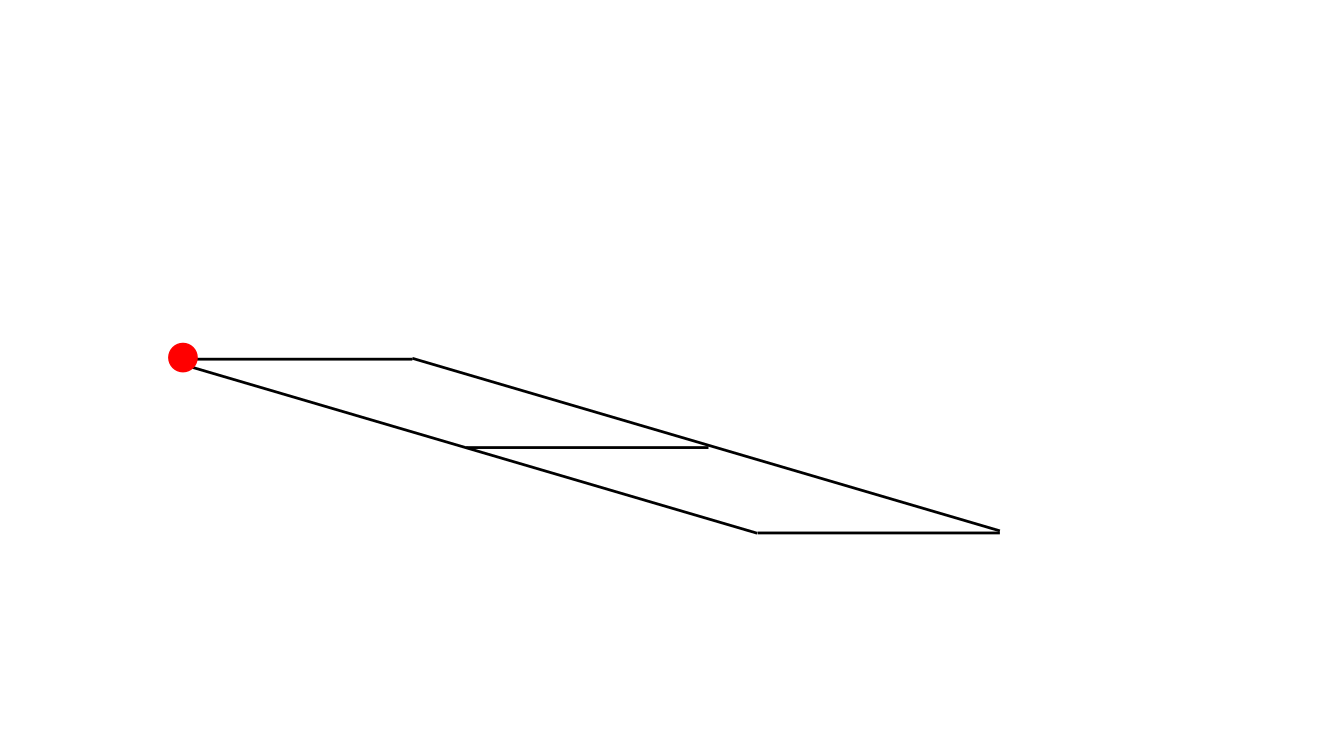
\includegraphics[width=2.8in]{figures/4dimensional4.png}}
    \caption{The idea of dimensionality reduction} 
  \label{fig:4dimensional} %% label for entire figure 
\end{figure}
After we transform the problem, then we can use the BVD-qG to solve the PBVD-qG. Let's now have a brief review of the BVD-qG. There are two agents exploring the graph: one is called exploring agent (EA) and one is called leader exploring agent (LEA). They follow the ``four step casual walk" to explore the graph. Before exploring a node $v=(x_1, \ldots, x_q) (1\leq x_i \leq d_i)$ from a node $u$, the shadowing agents(SA) move to the already explored neighbours of $v$ (the coordinate of the neighbours can be precisely computed). When EA visits the BV node (and is destroyed there), the LEA and the SAs are aware of the location of the new BV nodes. (the coordinates of them can be precisely computed) So, once the $v$ is identified, $2q$ agents surround each node $u\in N_{un}(v)$ and an additional agent enters it destroying the BV resident there and the instances that it generates. Note that in \cite{Cai}, the protocol BVD-qG use $3q+1$ agents, and because we view $d_1\times\ldots d_p$ agents as a ``big agent" then applying the BVD-qG protocol, so totally we need $d_1\times \ldots d_p\times (3q+1)$ agents.\\
We have map the $``d_1 \times \ldots \times d_p" (1\leq p\leq q)$ agents into one ``big agent". 
Assume that we employ a ``p dimensional" agent group (which contains $d_1 \times \ldots d_q$), then the coordinates of the agents are $(x_1, \ldots, x_p, \ldots, x_q)$, $(1\leq x_1\leq d_1, \ldots, 1\leq x_p\leq d_p, x_{p+1}=0, \ldots, x_q=0)$. Then the coordinates of the ``big agent" in the $q-p$ dimensional grid is $(x_{p+1},\ldots, x_q)$. The first p dimensional coordinates of the agents would not change in the whole exploring phase, but from $(p+1)^{th}$ dimensional coordinates, they make the same change as the ``big agent". More specifically, the $(p+1)^{th}$ of the agents make the same change as the first dimensional coordinate of the ``big agent"; the $(p+2)^{th}$ of the agents make the same change as the second dimensional coordinate of the ``big agent";\ldots. Assume that we now employ four agents(two agents are viewed as the LEA in the BVD-qG; two agents are viewed as the EA in the BVD-qG) to explore the 4-dimensional grid (they traverse the grid with the same routes following ``four step casual walk"), then the routes of the agents are as below (see Fig.\ref{fig:grouproute}):
\begin{figure} [H]
  \centering 
  \subfigure[The route of the ``big agent"(LEA in the BVD-qG)]{ 
    \label{fig:grouproute1:a} %% label for second subfigure 
    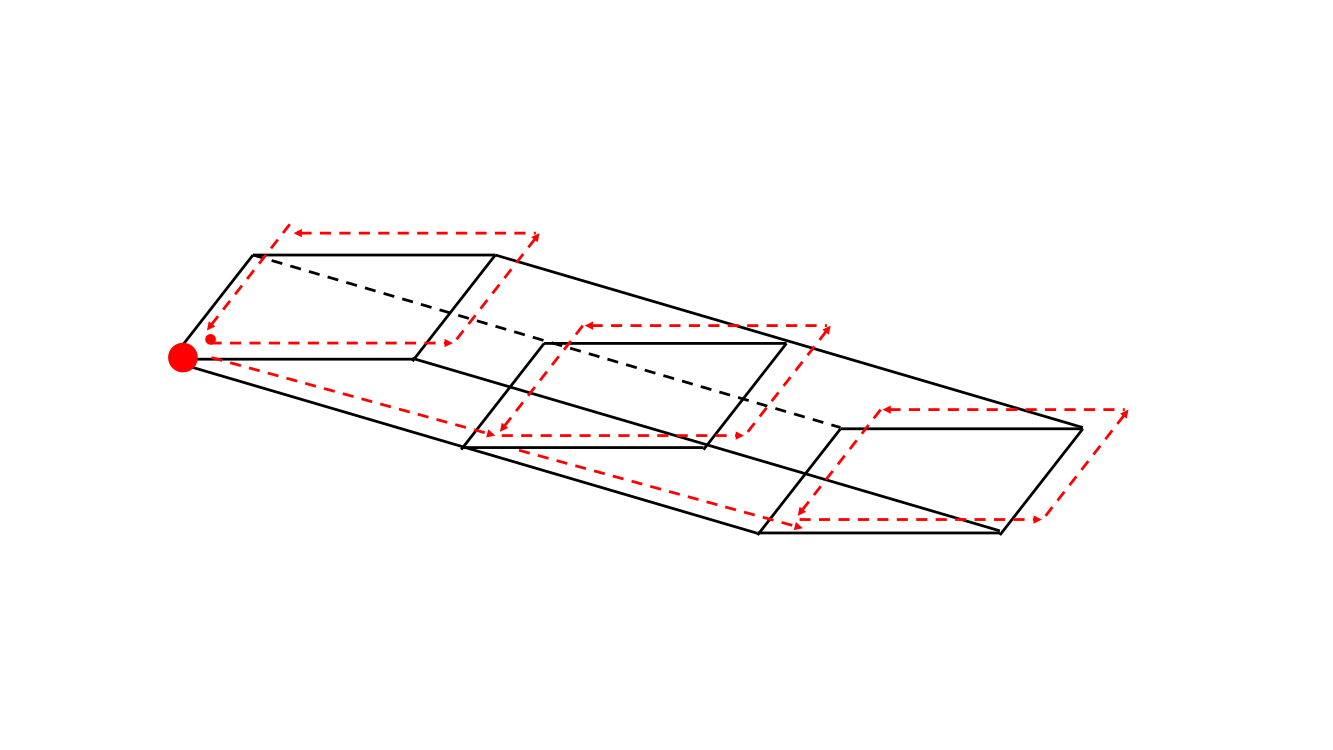
\includegraphics[width=3.5in]{figures/grouproute1.png}}
    \hspace{1in} 
\subfigure[The routes of the 2 agents viewed as the ``big agent"]{ 
    \label{fig:grouproute2:d} %% label for second subfigure 
    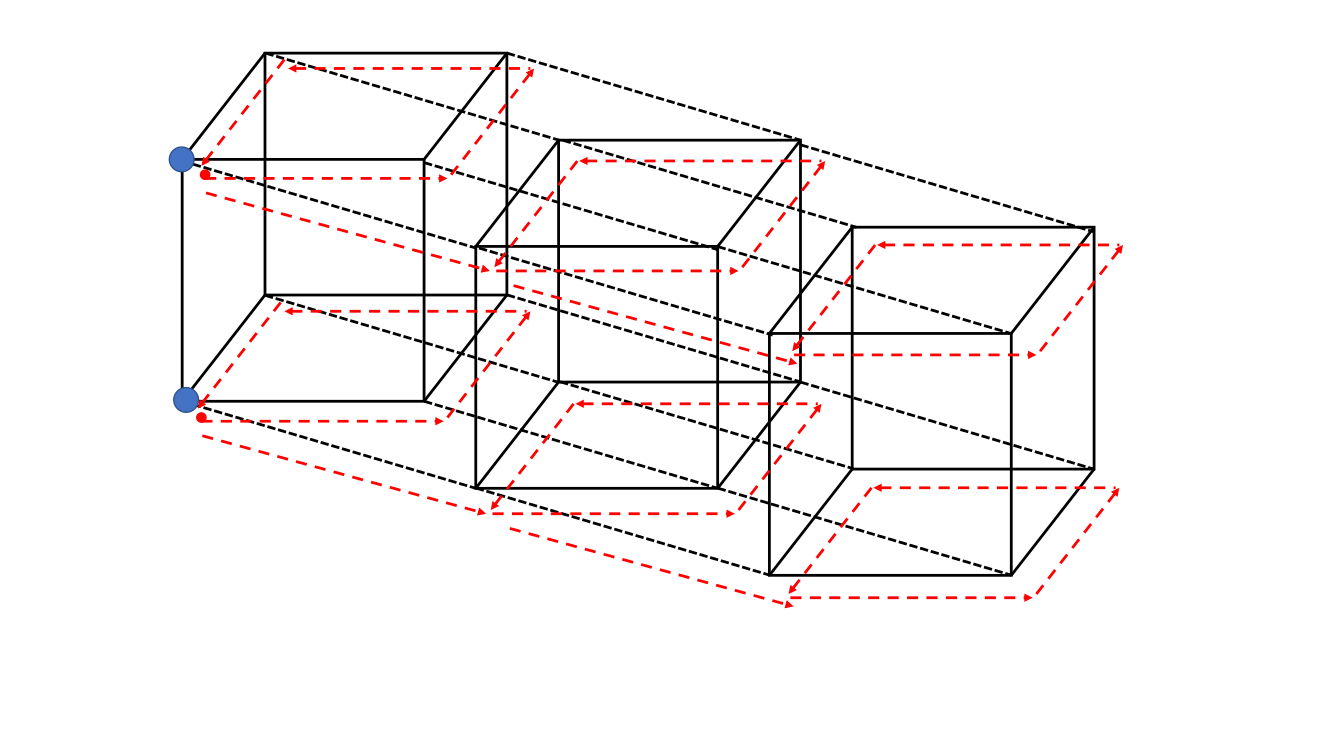
\includegraphics[width=3.5in]{figures/grouproute2.png}}
    \caption{The route of agent when exploring a $1\times1\times1\times2$ grid } 
  \label{fig:grouproute} %% label for entire figure 
\end{figure}

\noindent{\bf Analysis and Comparing}
Let's now compare the time cost, the number of movement and the casualties with different number of agents we employ. (Assuming that we are in a $d_1\times \ldots \times d_q$ q-dimensional grid)
Theorems in \cite{Cai} show us that the protocol BVD-qG performs a BV decontamination of a q-dimensional Grid using $3q+1$ agents and at most $q+1$ casualties with at most $O(qn)$ movements and $\Theta(n)$ time. Based on these theorems, we now discuss the number of agents, the casualties, the time cost and the number of movement in PBVD-qG.

\begin{theorem}
PBVD-qG performs a decontamination of a mesh (size of $n=d_1\times d_2(d_1>2,d_2>2)$ using $2\times d_1\times \ldots d_p (1\leq p\leq q)$ agents and at most $q-p+1$casualties, with at most $O(qn)$ and $\Theta(\frac{n}{d_1\times\ldots\times d_p})$ time.
\end{theorem}

\begin{proof}
In PBVD-qG, we can choose different number of agents to start the exploration, and that number results in different casualties and so on. Assuming that we use $2\times d_1\times \ldots d_p (1\leq p\leq q)$ agents to explore the graph, then actually we view $d_1\times \ldots d_p$ agents as a ``big agent", As we mentioned before, totally we need $d_1\times \ldots d_p\times (3q+1)$ agents (every $d_1\times\ldots d_p$ agents play the role of one agent in the BVD-qG). Now our problem changes into solving the BVD-qG problem in a $q-p$ dimensional grid with $d_{p+1}\times \ldots d_q$ agents, so the casualties and the times cost follow the same as the situation when we use BVD-qG in a $q-p$ grid. More specifically, the casualties are $q-p+1$ and the time is $\Theta(\frac{n}{d_1\times\ldots\times d_p})$. In BVD-qG, the number of movements by LEA, EA and each SA is $O(n)$ and since there are at most $q$ shadowing agents, the total number of movements until the BV is found is $O(qn)$ in the worst case. In PBVD-qG, the new ``n" should be $\frac{q\times d_1\times\ldots d_p\times n}{d_1\times\ldots\times d_p}$ the number of movement should be $O(qn)$.  
\end{proof}

\subsection{Tori}
%Informally, the torus is a mesh with "wrap-round" links that transform it into a regular graph. A torus of dimensions $d_1\times d_2$ has $n=d_1\times d_2$ nodes $v_{i,j} (1\leq i\leq d_1, 1\leq j\leq d_2)$ and each node has four neighbours which are $v_{i,j+1}, v_{i,j-1}, v_{i+1,j}, v_{i-1,j}. The algorithm to parallelly decontaminate the BV in a torus, called PBVD-T, follows a strategy very similar to the one used for the 2-dimensional grid described in section 5.2.1. There are two difference between the two strategies: 1) In 2-dimensional grid, all the agents move EAST in the exploration phase, while in the torus, because of the lack of borders, the spread of the BV might happen even if it reside in $v_{d_2, j}$ $(1\leq j\leq d_2)$, we place another group of agents at $v_{i,0}$ (i=0, 1, ? b-1) and these agents will stay here until the end of exploration phase. 2) 
%Initially, 2 $d_1$ agents are place at $v_{0,i}$, $v{1,i}$ (i=0,1, ?d_2-1) (first round). If no agents are destroyed, then we start the safe-exploration phase. If one of the agents is destroyed, assuming that the original BV resides in node $v{0,j}$, $(1\leq j\leq d_1)$, then all the clones of the BV are destroyed. If the BV resides in node $v{1,j}$, $(1\leq j\leq d_1)$, then the elimination phase begin.             

\ref{fig:grouproute}):
\begin{figure} [H]
  \centering 
  \subfigure[The route of the ``big agent"(LEA in the BVD-qG)]{ 
    \label{fig:grouproute1:a} %% label for second subfigure 
    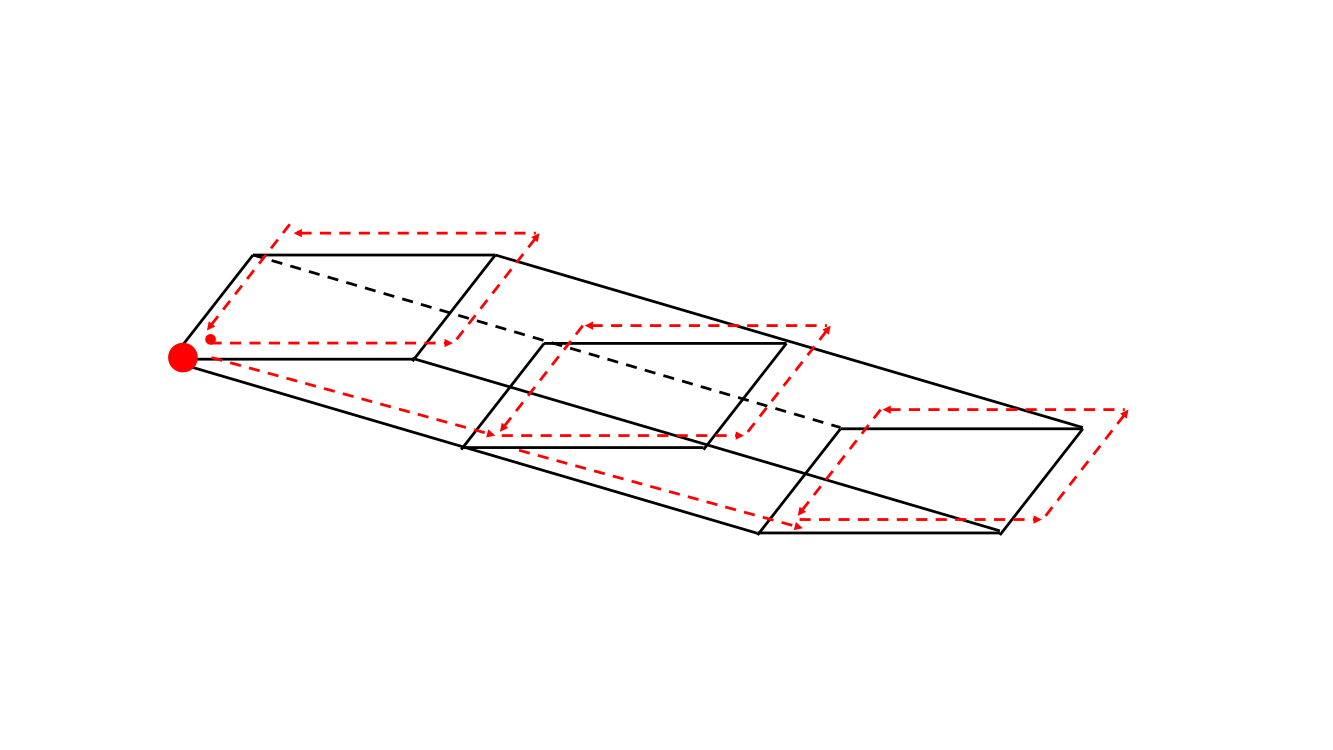
\includegraphics[width=3.5in]{figures/grouproute1.png}}
    \hspace{1in} 
\subfigure[The routes of the 2 agents viewed as the ``big agent"]{ 
    \label{fig:grouproute2:d} %% label for second subfigure 
    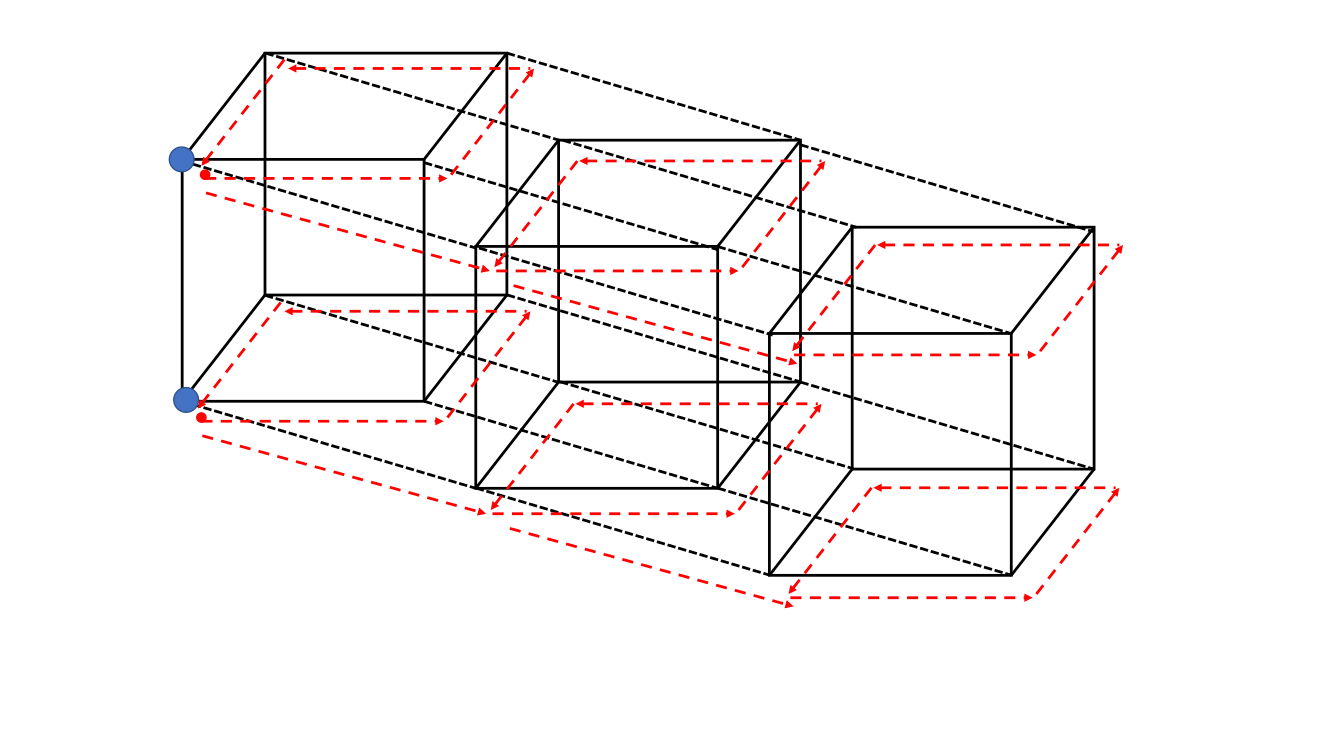
\includegraphics[width=3.5in]{figures/grouproute2.png}}
    \caption{The route of agent when exploring a $1\times1\times1\times2$ grid } 
  \label{fig:grouproute} %% label for entire figure 
\end{figure}








